% Created 2014-04-11 Fri 07:14
\documentclass[a4paper,12pt]{report}
\usepackage[utf8]{inputenc}
\usepackage[T1]{fontenc}
\usepackage{fixltx2e}
\usepackage{graphicx}
\usepackage{longtable}
\usepackage{float}
\usepackage{wrapfig}
\usepackage{rotating}
\usepackage[normalem]{ulem}
\usepackage{amsmath}
\usepackage{textcomp}
\usepackage{marvosym}
\usepackage{wasysym}
\usepackage{amssymb}
\usepackage{hyperref}
\tolerance=1000
\usepackage{minted}
\usepackage[bibstyle=numeric,citestyle=numeric,backend=biber]{biblatex}
\addbibresource{bibliography.bib}
\usepackage[]{hyperref}
\usepackage{caption}
\usepackage{subcaption}
\usepackage{rotating}
\hypersetup{hidelinks}
\usepackage[]{nomencl}
\usepackage{svg}
\usepackage{xspace}
\usepackage{dirtree}
\usepackage[autostyle]{csquotes}
\definecolor{dhscodebg}{rgb}{0.95,0.95,0.95}
\usepackage{menukeys}
\usepackage{scalefnt}
\usepackage{wrapfig}
\usepackage{lscape}
\usepackage{rotating}
\usepackage{epstopdf}
\newcommand{\mypddl}{\smallerft[0.8]{myPDDL}\xspace}
\newcommand{\pddlstudio}{\textsc{pddl studio}\xspace}
\newcommand{\itsimple}{\textsc{itSimple}\xspace}
\newcommand{\pddlmode}{\textsc{pddl}-mode\xspace}
\newcommand{\pddl}{\textsc{pddl}\xspace}
\newcommand{\uml}{\textsc{uml}\xspace}
\newcommand\smallerft[2][0.85]{{\scalefont{#1}#2}}
\author{Volker Strobel}
\date{\today}
\title{My\textsc{pddl} - A Modular Knowledge Engineering System for the Planning Domain Definition Language}
\hypersetup{
  pdfkeywords={},
  pdfsubject={},
  pdfcreator={Emacs 24.3.1 (Org mode 8.2.5h)}}
\begin{document}

\maketitle
\tableofcontents

\begin{abstract}
Writing and maintaining planning problems, specified in the widely
used \emph{Planning Domain Definition Language} (\textsc{pddl}), can be
difficult, time-consuming and error-prone. This thesis will present
\mypddl, a toolkit that helps knowledge engineers to develop,
visualize and manipulate \pddl planning task specifications. With
\mypddl, structured \pddl projects can be created and edited using
code templates and syntax highlighting. One tool visualizes the type
hierarchy in \pddl domains, allowing knowledge engineers to understand
the representation structure at a glance and to also keep track of
developments with a basic revision control system. Another tool allows
calculating distances between objects specified by predicates in a
problem file. These tools make use of an interface that provides a
general way for reading and writing \pddl specifications by using the
programming language Clojure, and thus presenting a means of bypassing
\pddl's limited modeling capacity. They are made accessible in the
customizable editor Sublime Text. A small user study, conducted with
eight inexperienced \pddl users, shows some initial evidence that the
syntax highlighting feature and the automated creation of type
diagrams could support knowledge engineers in the design and analysis
process. The users detected 35 \% more errors using the syntax
highlighter in the same time as non-users and the average task
completion time for questions on a hierarchical domain was reduced by
52 \%.
\end{abstract}

\chapter{Introduction}
\label{sec-1}
\label{ch:introduction}

Have you ever struggled to find the optimal sequence of actions for a
recurrent problem? While a task like this could take you hours, weeks
or even a lifetime to complete, a planning software could possibly get
the job done within milliseconds. Being a key aspect of artificial
intelligence, planning is concerned with devising a plan, i.e. a
sequence of actions, to achieve a desired goal
\cite{helmert2008understanding}. It can be both a tool to create
automated systems and a means to support and understand human behavior
\cite{konar1999artificial}. However, the effectiveness of planning
largely depends on the quality of the problem formalization
\cite{shah2013knowledge,keps2014}. To ensure a standardized modeling
format, the Planning Domain Definition Language (\textsc{pddl})
\cite{mcdermott1998pddl} was developed and has become the de facto
standard for the description of planning tasks
\cite{ilghami2005extension}. The discipline that deals with the
integration of world information into a computer system via a human
expert is called knowledge engineering \cite{feigenbaum1983fifth}.
While automated planning could save you a vast amount of time if
everything works as intended, creating the planning task
specifications is a complex task that can be error-prone and
cumbersome. Searching for an error in a long \pddl file can be like
looking for a needle in a haystack; debugging could take hours as some
planners crash on erroneous \pddl files without providing any problem
report.

The strenuous modeling process and the efficiency issues it brings
gave rise to the need for tools designed for creating planning task
specifications \cite{shah2013knowledge}, so much so that the annual
International Conference on Automated Planning and Scheduling \footnote{More information on \textsc{icaps} 2014, the 24th
International Conference on Automated Planning and Scheduling can be
found on \url{http://icaps14.icaps-conference.org/}.} has
workshops (such as Knowledge Engineering for Planning and Scheduling),
tutorials and presentations dedicated to this topic. Therefore,
developing such tools for \pddl and hence facilitating the knowledge
engineering process is appreciated and worthwhile.

The modular toolkit \mypddl (\textit{m}odeling efficientl\textit{y}
\pddl was developed, within the scope of this thesis, in order to
tackle frequent needs of knowledge engineers, like project management,
efficient development, error-detection, team collaboration and to
increase the acceptance and usage of \pddl in real-world domains
\cite{shah2013knowledge,keps2014}.

\mypddl is intended to support knowledge engineers throughout the
entire design cycle of specifying planning tasks. In the initial
stages, it allows for the creation of structured \textsc{pddl}
projects that should encourage a disciplined design process. With the
help of snippets, i.e. code templates, often used constructs can be
inserted in \textsc{pddl} files. A syntax highlighting feature that
speeds up the error-detection can come in handy in intermediate
stages. Understanding the textual representation of complex type
hierarchies in domain files can be confusing, so an additional feature
enables their visualization. \textsc{pddl}'s limited modeling
capabilities were bypassed by developing an interface that converts
\textsc{pddl} code into Clojure \cite{hickey2008clojure} code and vice
versa. Within this project, the interface was employed for a feature
that calculates distances between objects specified in a problem
model, but the interface provides numerous other possibilities and
could also be used to further automate the modeling process. All of
these features were integrated into the customizable and extensible
Sublime Text \cite{sublimetext2} editor. Since the main aim in the
development of the toolkit was for it to be easy to use and maintain,
it is evaluated with regard to these criteria. The usability was
assessed by means of a user test with eight subjects that had no prior
experience with artificial intelligence planning. The results indicate
that both error-detection and the understanding of a given domain can
be facilitated by \mypddl.

To lay the foundations for this thesis, a basic introduction to and
design principles for \pddl will be given in Chapter \ref{ch:basics}.
Existing tools will be critically reviewed in Chapter \ref{ch:related} to
set the goals for \mypddl. The features and modules of \mypddl are then
described in detail in Chapter \ref{ch:tools}. Details and results of the
usability study are provided in Chapter \ref{ch:evaluation}. Finally, the
implications are briefly discussed before an outlook for future
research and developments in the field concludes this thesis in
Chapter \ref{ch:conclusion}.
\chapter{Background and Basics}
\label{sec-2}
\label{ch:basics}

The human brain is an astonishing structure that allows us to get by
in a highly complex world and give more or less rational reasons for
our past or planned actions. While computer systems are yet to fully
master these skills, the study of artificial intelligence tries to
narrow this gap \cite{akerkar2012intelligent}. For this purpose,
constructs are needed that can represent the information about the
world and the problem. In automated planning, this is usually done
\cite{fox2003pddl2} using a planning language, like \textsc{pddl}.

To illustrate the usage and basics of \textsc{pddl}, the remainder of
this section presents a modeling walkthrough using a fictional
example.

Consider the following world that is to be integrated into a computer
system using \textsc{pddl}:

\begin{quote}
\emph{Hacker World} \\
If hackers are hungry, they have to eat some pizza in order to be able
to work, that is to exploit (or hack into) vulnerable software.
\end{quote}
In this description, we can identify several constructs that should
somehow be integrated into the computer. There are:

\begin{description}
\item[{Types of entities: }] The world consists of hackers, software and
pizza.
\item[{Logical states:}] Hackers can be hungry or not, software can be
vulnerable or not, software can be exploited or not.
\item[{Actions:}] Hackers can exploit software and they can eat pizza.
\end{description}
This description of a world can be specified in \textsc{pddl} using a
domain file. The domain file can be compared to a stage setting,
providing the framework for a specific problem scenario by way of
general, abstract constructs and conditions.

In the world of hackers and pizzas, such a domain specific problem
could be:

\begin{quote}
\emph{Gary's Huge Problem} \\
Gary is a hungry hacker who should somehow exploit the vulnerable
software MagicFailureApp. Some pepperoni pizza is lying around.
\end{quote}
Again, several constructs can be identified:

\begin{description}
\item[{Objects}] The hacker Gary (in \textsc{pddl} all entities are
objects, including persons), the pepperoni pizza, the
software.

\item[{Initial state}] Gary is hungry and the software MagicFailureApp
is vulnerable.

\item[{Goal state}] The MagicFailureApp is exploited.
\end{description}
Assume that Gary wants the help of an automated planning system to
plan the sequence of required actions (\emph{Who has to eat pizza?}, \emph{What
should be hacked?} and \emph{In what order should these things be done?}),
leading from the initial state to the goal state. These specifications
must be formalized so that a planner can utilize them. In
\textsc{pddl}, this is done in problem files. In the end, Gary will be
able to feed the domain and the problem file into a planner which will
generate a sequence of actions that Gary can take to solve his
problem.

Summing up, \textsc{pddl} planning tasks specifications
are composed of two separate, corresponding files:

\begin{description}
\item[{Domain file:}] General, problem-independent description of types,
predicates (logical states) and actions.

\item[{Problem file:}] Specification of a concrete problem within a
particular domain, expressed by the initial state
and the goal state. Specific values are assigned to
the templates provided by the domain file
(instantiation).
\end{description}
This separation allows for a powerful task modeling process: while
general world information is described in the domain file, specific
instances of problems are created in the problem files. This means
that one abstract model of a world can be used for solving many
problem instances.

The rest of this section is to propose general design guidelines for,
and give an introduction to \textsc{pddl} \footnote{More complete descriptions of \textsc{pddl}, as well as
formulations in Backus-Naur form (BNF) are provided by
\textcite{fox2003pddl2} for \textsc{pddl} 2.2 and
\textcite{kovacs2011bnf} for \textsc{pddl} 3.1.}, to serve as a basis
for the rest of this thesis. To this end, the syntax of common
constructs of domain and problem files is further investigated in a
step-by-step approach, continuing with the above described example.

\section{Analysis}
\label{sec-2-1}

How do you begin to model a planning task? The first, and possibly
most significant step to integrate information into a computer system,
is gaining an \emph{understanding} of the problem
\cite{polya2008solve,helmert2008understanding}. For modeling in
\textsc{pddl}, the following six general design principles \footnote{These design principles are based on
\citetitle{felleisen2010design} that describes four steps of designing
class hierarchies for object-oriented programs.} ought to
lead to a thorough, stepwise, and iterative modeling process:

\begin{description}
\item[{Analysis:}] Every task specification should begin with an analysis
of the informal world and the problem statement. In
this design step, one determines relevant types,
adequate examples and identifies both the initial and
the goal state.

\item[{Type diagram:}] Based on the preceding analysis, the relationship
of the identified categories or types is
represented, using a diagram. This can be done on
paper or with the help of a graph editor.

\item[{Domain definition:}] In this step, the diagrams are translated into
\textsc{pddl}. Furthermore predicates and actions are declared.

\item[{Problem definition:}] After completing the domain definition,
objects can be instantiated in the problem file. The initial and
goal states are modeled using the predicates declared in the
domain file.

\item[{Planning:}] Now, one can provide the domain and problem definition
to a planner. The planner then generates a plan, i.e. a
sequence of actions that leads to the goal state.

\item[{Plan analysis:}] Finally, the generated plan needs to be inspected.
If any design mistakes or inconistencies are
detected, it is advisable to restart at an earlier
design step.
\end{description}

The following two sections deal with the creation of a domain and
problem definition. At the end of the introduction of each construct,
the corresponding code block of the \emph{Hacker World} and \emph{Gary's Huge
Problem} is given.
\section{Domain File}
\label{sec-2-2}

The domain file sets the framework for planning tasks. It models the
world in which the problem occurs and hence determines which types and
predicates are available and which actions are possible.

\subsection{Domain Definition}
\label{sec-2-2-1}

We begin with the definition of the domain file. Every domain file
starts with \texttt{(define (domain DNAME) ...)}, where \texttt{DNAME} specifies the
name of the domain. A semicolon (\texttt{;}) declares the rest of the line as
comment.

\begin{listing}[H]
\begin{minted}[fontsize=\small,bgcolor=dhscodebg,rulecolor=\color{gray!40},frame=lines,framesep=5\fboxrule,framerule=1pt,tabsize=2]{text}
; Hacker World - A realistic example
(define (domain hacker-world)
\end{minted}
\caption{The domain definition of the \emph{Hacker World}}
\end{listing}
\subsection{Requirements}
\label{sec-2-2-2}

\pddl is composed of feature subsets \cite{mcdermott1998pddl}.
As most planners only support some of these subsets, the requirements
block is useful for a planner to determine if it can act on a given
problem. While basic specifications are used by default
\cite{mcdermott1998pddl}, further requirements have to be stated
explicitly. For example, one requirement used by many planning domains
\cite{wickler2011using} is:

\begin{description}
\item[{:typing}] Enables the typification of variables (see
\ref{subsubsec:types} Types below), so that it is mandatory for
variables to be of a particular type.
\end{description}

Besides \texttt{:typing}, the \emph{Hacker World} will use a further
requirement:

\begin{description}
\item[{:negative-preconditions}] Allows for the specification of negative
preconditions in actions, so that an action can only be executed
if a predicate is not true initially.
\end{description}

\begin{listing}[H]
\begin{minted}[fontsize=\small,bgcolor=dhscodebg,rulecolor=\color{gray!40},frame=lines,framesep=5\fboxrule,framerule=1pt,tabsize=2]{text}
(:requirements :typing
               :negative-preconditions)
\end{minted}
\caption{The requirements that are necessary to model the \emph{Hacker World}}
\end{listing}
\subsection{Types}
\label{sec-2-2-3}
\label{subsubsec:types}
Often in the real-world, there will be individual objects of the same
kind or type. There may be many different desks, but all share
common properties, like having a flat upper surface, and all are
pieces of furniture.

\pddl allows for declaring types and thereby structuring the
domain in the \texttt{(:types ...)} block. Relations can be expressed with a
type hierarchy, in which any type can be a subtype of yet another
type. Typed lists are used to assign types to variables.
Parameters in actions, as well as arguments in predicates can be typed
in this manner. Later, in the problem file, objects are assigned to
types. Types are declared using a list of strings, followed by a
hyphen (\texttt{-}), followed by the higher-level type. Every \pddl
domain includes the built-in types \texttt{object} and \texttt{number}, and every
defined type, in turn, is a subtype of \texttt{object}.

\begin{listing}[H]
\begin{minted}[fontsize=\small,bgcolor=dhscodebg,rulecolor=\color{gray!40},frame=lines,framesep=5\fboxrule,framerule=1pt,tabsize=2]{text}
(:types hacker non-hacker - person
        desk chair - furniture
        laptop workstation - computer
        pizza burgers fries - food
        pepperoni supreme - pizza
        person furniture compiter food software - object)
\end{minted}
\caption{The type hierarchy for the \emph{Hacker World}, consisting of different types of persons, furniture, computers, hackers, food, pizza and software. The elements on the left-hand side (for example \texttt{hacker non-hacker}) are declared subtypes of the right-hand side (\texttt{person}) whereby the type hierarchy is expressed.}
\end{listing}
\subsection{Predicates}
\label{sec-2-2-4}

How can we describe properties of objects and states of the world?
Predicates are templates to represent logical facts and can be either
true or false. In the \texttt{:(predicates ...)} block, predicate names and
the number of arguments together with the corresponding types are
declared. The general syntax for a predicate is \texttt{(pname ?v1 - t1 ?v2 -
t2 ...)}, where \texttt{?} followed by a name (\texttt{v1}, \texttt{v2}) declares a
variable, and the expression (\texttt{t1}, \texttt{t2}) following the hyphen (\texttt{-})
states the type of this variable. All the types that are used must be
declared in the typing section first. The number of variables (or
arguments) determines the arity of a predicate ranging from zero
(nullary predicate) to any positive integer (n-ary predicate). Type
assignments for variables that have the same type and are declared
side by side can be grouped, meaning that \texttt{(p ?v1 - t ?v2 - t)} is
equivalent to \texttt{(p ?v1 ?v2 - t)}.

\begin{listing}[H]
\begin{minted}[fontsize=\small,bgcolor=dhscodebg,rulecolor=\color{gray!40},frame=lines,framesep=5\fboxrule,framerule=1pt,tabsize=2]{text}
(:predicates (has ?s - software ?p - person)
             (hungry ?p - person)
             (vulnerable ?s - software)
             (exploited ?s - software)
             (distance ?o1 ?o2 - object ?x - number)
             (location ?o - object ?x ?y - number))
\end{minted}
\caption{This section declares five predicates: the unary predicates \texttt{hungry}, \texttt{vulnerable} and \texttt{exploited}, the binary predicate \texttt{has}, and the 3-ary predicates \texttt{location} that specifies x and y coordinates for objects, \texttt{distance} that expresses the distance between objects.}
\end{listing}
\subsection{Actions}
\label{sec-2-2-5}

Now that we have predicates for describing world states, we still need
a means for changing their value. This is done with action. Actions
are operators in \textsc{pddl}, because they can change properties of
objects by changing predicate values, so that problems can be solved.
Actions usually consist of three parts:

\begin{description}
\item[{:parameters}] A (typed) argument list that determines which
variables can be used in the precondition and effect
part.

\item[{:precondition}] A combination of predicates, all of which must be
true before an action can be executed. Therefore,
this part describes the applicability of an action.

\item[{:effect}] Specifies the new values of the declared predicates, once
the action has been completed. Therefore, it describes
the post-condition of an action.
\end{description}

\begin{listing}[H]
\begin{minted}[fontsize=\small,bgcolor=dhscodebg,rulecolor=\color{gray!40},frame=lines,framesep=5\fboxrule,framerule=1pt,tabsize=2]{text}
;; Eat a delicious pizza
(:action eat-pizza
  :parameters (?pi - pizza ?p - person)
  :precondition (and (hungry ?p)
                     (has ?pi ?p))
  :effect (and (not (hungry ?p))
               (not (has ?pi ?p))))

;; Exploit vulnerable software of a victim
(:action exploit        
  :parameters (?h - hacker ?s - software ?p - person)
  :precondition (and (has ?s ?p)
                     (vulnerable ?s)
                     (not (hungry ?h)))
  :effect (exploited ?s))

;; Move a piece of furniture
(:action move
  :parameters (?f - furniture ?old-x ?old-y ?new-x ?new-y)
  :effect (and (location ?f ?new-x ?new-y)
               (not (location ?f ?old-x ?old-y)))))
\end{minted}
\caption{Three actions that can change logical values in the \emph{Hacker World}. It is important to remember that predicate values keep being true if an effect adds a logical fact. This is often not desired. Consider the action move, that changes the location of a chair. Only having the effect \texttt{(location chair ?new-x ?new-y)} would result in the chair being located at two locations, at \texttt{?old-x} and \texttt{?old-y} and the new, specified coordinates. Therefore, the old coordinates have to be deleted, using \texttt{(not ...)}. The \texttt{:precondition} part can be omitted, if an action should be always applicable.}
\end{listing}
\section{Problem File}
\label{sec-2-3}

A planning problem consists of a domain and a corresponding problem
file. Within problem files, concrete objects are created
(instantiated). Furthermore, the initial world state and the desired
goal state that is to be reached are declared.

\subsection{Problem Definition}
\label{sec-2-3-1}

Analogous to the domain definition, problem files are initiated with
\texttt{(define (problem PNAME) ...)}, where \texttt{PNAME} declares the name of the
problem.

\begin{listing}[H]
\begin{minted}[fontsize=\small,bgcolor=dhscodebg,rulecolor=\color{gray!40},frame=lines,framesep=5\fboxrule,framerule=1pt,tabsize=2]{text}
(define (problem garys-huge-problem)
\end{minted}
\caption{Initiating the problem file with the name garys-huge-problem}
\end{listing}
\subsection{Associated Domain}
\label{sec-2-3-2}

Problems occur in worlds. Therefore, problem files are designed with
regard to domain files that need to be referenced at this point in the
problem file. This means that \texttt{DNAME} in \texttt{(:domain DNAME)} and \texttt{DNAME}
in \texttt{(define (domain DNAME) ...)} in the corresponding domain file have
to be identical.

\begin{listing}[H]
\begin{minted}[fontsize=\small,bgcolor=dhscodebg,rulecolor=\color{gray!40},frame=lines,framesep=5\fboxrule,framerule=1pt,tabsize=2]{text}
(:domain hacker-world)
\end{minted}
\caption{The domain "hacker-world" is the corresponding domain name to the problem garys-huge-problem}
\end{listing}

\subsection{Objects}
\label{sec-2-3-3}

Since types are only empty shells, they need to be instantiated. This
is done in the \texttt{(:objects ...)} block. Instantiating types means that
concrete objects are assigned to the types.

\begin{listing}[H]
\begin{minted}[fontsize=\small,bgcolor=dhscodebg,rulecolor=\color{gray!40},frame=lines,framesep=5\fboxrule,framerule=1pt,tabsize=2]{text}
(:objects big-pepperoni - pepperoni
          gary - hacker
          gisela - non-hacker
          magicfailureapp - software)
\end{minted}
\caption{This part assigns concrete objects to the type templates. In this case, magicfailureapp - software means that the object magicfailureapp is of the type application.}
\end{listing}

\subsection{Init}
\label{sec-2-3-4}

The \texttt{(:init ...)} block models the initial state of the world with a
list of instantiated predicates that are declared as true. All other,
non-specified predicates are assumed to be false. This is called the
\emph{closed-world assumption} \footnote{By specifying \texttt{:open-world} in the requirements part, \textsc{pddl} is
also capable of using the open world assumption, where non-specified
predicates can be both, true or false.}.

\begin{listing}[H]
\begin{minted}[fontsize=\small,bgcolor=dhscodebg,rulecolor=\color{gray!40},frame=lines,framesep=5\fboxrule,framerule=1pt,tabsize=2]{text}
(:init (hungry gary)
       (has big-pepperoni gary)
       (vulnerable magicfailureapp)
       (has magicfailureapp gisela))
\end{minted}
\caption{The initial situation in Gary's Huge Problem consists of the hungry hacker Gary and the vulnerable application MagicFailureApp that belongs to Gisela.}
\end{listing}

\subsection{Goal}
\label{sec-2-3-5}

The goal state is described by the logical fact that is desirable and
should be reached with the execution of the plan. In \textsc{pddl},
several goals are combined with \texttt{(and ...)}. All unspecified predicates
are irrelevant, meaning that they can be either true or false in the
goal state.

\begin{listing}[H]
\begin{minted}[fontsize=\small,bgcolor=dhscodebg,rulecolor=\color{gray!40},frame=lines,framesep=5\fboxrule,framerule=1pt,tabsize=2]{text}
(:goal (exploited magicfailureapp))
\end{minted}
\caption{In the end, the software magicfailureapp should be exploited.}
\end{listing}

\section{Planning}
\label{sec-2-4}

Finally, the effort of the formalization of the planning task will be
rewarded with the automatic generation of a plan. There is a broad
range of available planners \footnote{For an overview of planners that participated in the 2011
International Planning Competition and their features, see
\url{http://www.plg.inf.uc3m.es/ipc2011-deterministic/ParticipatingPlanners.html}.}. However, most planners only
support certain subsets of \pddl and have some
peculiarities \footnote{A short discussion on planners and their "excentricities" can
be found at \url{http://users.cecs.anu.edu.au/~patrik/pddlman/writing.html}.}. Additionally, the quality of error messages is
very diverse, ranging from stating that an error occurred to
displaying line number and found problem.

This thesis uses the planner SGPlan\(_{\text{5}}\) \cite{hsu2008sgplan}, a planner
that supports many \textsc{pddl} features and has comprehensive
error messages that state the actual problem \footnote{Additionally, SGPlan\(_{\text{5}}\) was the winner of the 1st Prize
Satisficing Planning in the Deterministic Part of the International
Planning Competition (IPC) in 2006
\url{http://zeus.ing.unibs.it/ipc-5/results.html}.}.

The planner SGPlan\(_{\text{5}}\) can be used by specifying the domain file and
the problem file in a command line interface.

The relevant output lines for \emph{Gary's Huge Problem}, specified in the
\emph{Hacker World} look as follows:
\vspace*{0.2cm}

\begin{minted}[fontsize=\small,bgcolor=dhscodebg,rulecolor=\color{gray!40},frame=lines,framesep=5\fboxrule,framerule=1pt,tabsize=2]{text}
0.001: (EAT-PIZZA BIG-PEPPERONI-PIZZA GARY) [1]
1.002: (EXPLOIT GARY MAGICFAILUREAPP GISELA) [1]
\end{minted}

The numbers to the left (\texttt{0.001}, \texttt{1.002}) and to the right (\texttt{[1]})
specify the start time and the duration of the actions, respectively.
Since we did not use any timestamps, they are dispensable in this
case, because only the order of actions is relevant.

Gary now definitely knows that he first has to eat the pepperoni pizza
before he can exploit Gisela's application MagicFailureApp.

Since specifying \textsc{pddl} files can be time-consuming the next
chapter will compare knowledge engineering tools that support the user
in effectively eneffective planning model.

\chapter{Related Work}
\label{sec-3}
\label{ch:related}

This chapter is to introduce knowledge engineering tools that allow
editing \textsc{pddl} files in a textual environment to some extent.
All tools provide features to support the user in writing correct
\textsc{pddl} code more efficiently. After introducing the tools, they
are compared and their shortcomings are discussed to set the stage for
\mypddl.

\section{PDDL Studio}
\label{sec-3-1}

\pddlstudio \cite{chomuttool,plch2012inspect} is an application for
creating and managing \textsc{pddl} projects, i.e. a collection of
\textsc{pddl} files. The \pddlstudio integrated development
environment (IDE) was inspired by Microsoft Visual Studio
\cite{visstudio} and imperative programming paradigms. Its main
features are syntax highlighting, error detection, context sensitive
code completion, code folding, project management, and planner
integration. Many of these features are based on a parser, which
continuously analyzes the code and divides it into syntactic elements.
These elements and the way in which they relate to each other can then
be identified. The syntax highlighter is a tool that colors constructs
according to their syntactical meaning within the code. In the case of
\pddlstudio, it colors names, variables, errors, keywords, predicates,
types and brackets each in a different customizable color.
\pddlstudio's error detection can recognize both syntax errors
(missing keywords, parentheses, etc.) and semantic errors (wrong type
of predicate parameters, misspelled predicates, etc.). Since semantic
errors can be of an interfile nature, meaning that there is a mismatch
between domain and problem file, \pddlstudio can detect such errors in
real time. The code completion feature allows for the selection of
completion suggestions for standard \textsc{pddl} constructs as well
as for terms that have been used before within this file or other
files in the same project. Code folding allows the knowledge engineer
to hide certain code units or blocks that are currently not needed.
Only the first line of the block is then displayed. \pddlstudio's code folding feature works on the basis of syntax. This means
that it can tell different code blocks apart with the help of the
parser and is thus able to fold the code accordingly. All these above
mentioned features of \pddlstudio utilize the parser. Another
important feature of the \pddlstudio project is a project
manager. This keeps track of all files, displays them in a tree
structure, saves them upon compilation and is also necessary for the
interfile error detection and code completion functionalities. Lastly,
a command-line interface allows the integration of planners in order
to run and compare different planning software.
\section{itSIMPLE}
\label{sec-3-2}

Unlike \pddlstudio, which provides a text based editor for \pddl, the
\itsimple \cite{vaquero2005itsimple} editor has, as its main feature, a
graphical approach that allows for designing planning tasks in an
object-oriented approach using Unified Modeling Language (\textsc{uml})
\cite{booch1999unified} diagrams. \textsc{uml} was invented in order
to standardize modeling in software engineering (SE) and the latest
version (\textsc{uml} 2.4.1) \cite{umllatest} consists of 14 different types of diagrams
divided into two larger groups: structure and behavior diagrams. In
the process leading up to \itsimple, \textsc{uml.p} (\textsc{uml} in a
Planning Approach) was proposed, a \textsc{uml} variant specifically
designed for modeling planning domains and problems
\cite{vaquero2006use}.

This variant specifies:

\begin{itemize}
\item Class Diagrams for static domain features
\item Object Diagrams to describe the initial and the goal state in
problem specifications
\item StateChart Diagrams to represent dynamic characteristics such as
actions in domain specifications.
\end{itemize}

Thus, \itsimple uses both \textsc{uml} structure diagrams (Class and
Object Diagrams) and \textsc{uml} behavior diagrams (StateChart
Diagrams). The main purpose of \itsimple is supporting knowledge
engineers in the initial stages of the design phase by making tools
available that help with the transition from the informality of the
real world to the formal specifications of domain models. The
professed aim of the project is to provide a means to a
\enquote\{disciplined process of elicitation, organization and analysis
of requirements\} \cite{vaquero2005itsimple}. However, subsequent
design stages are also supported. Once domain and problem models have
been created, \textsc{pddl} representations can be generated from the
UML.P diagrams, edited, and then used as input to a number of
different integrated planning systems. Therefore, one of the tools
already introduced within the scope of \pddlstudio, planner
integration, is also implemented. However, unlike in \textsc{pddl}
Studio, \itsimple has a more user-friendly approach to planner
integration: domain and problem can be fed to the planner with the
press of a button, while in \textsc{pddl} Studio, the user has to know
and input commands in a command-line interface.

Not only is it possible to directly input the domains and problems
into a planner, another tool can inspect the output from the planning
system using the built-in plan analysis. This consists of a plan
visualization that shows the interaction between the plan and the
domain by highlighting every change caused by an action. \itSimple's
modeling workflow is unidirectional, as changes in the \textsc{pddl} domain do
not affect the UML model and UML models have to be modeled manually,
meaning that they cannot by generated using \textsc{pddl}. Starting in version
4.0 \cite{vaquero2012itsimple4} \itsimple expanded its features to
allow the creation of \textsc{pddl} projects from scratch (i.e. without UML to
\textsc{pddl} translation process). Thus far, the \textsc{pddl} editing features are
basic. A minimal syntax highlighting feature recognizes \textsc{pddl} keywords,
variables, and comments. Furthermore, \itsimple provides templates for
\textsc{pddl} constructs, such as requirement specifications, predicates,
actions, initial and goal definitions.
\section{PDDL-Mode for Emacs}
\label{sec-3-3}
GNU Emacs is a text editor, primarily written in, and customizable by
using Emacs Lisp, a Lisp dialect
\cite{stallman1981emacs,lewis1990gnu}. The core values of Emacs are
its extensibility and customizability. \pddlmode \cite{pddlmode} is a
major Emacs mode, which determines the editing behavior of Emacs, for
browsing and editing \textsc{PDDL} files. It provides syntax
highlighting by way of basic pattern matching of keywords, variables
and comments. Additional features are automatic indentation and code
completion as well as bracket matching. Code snippets for the creation
of domains, problems and actions are also available. Finally, the
\pddlmode keeps track of action and problem declarations by adding
them to a menu and thus intending to allow for easy and fast code
navigation.
\section{Critical Review}
\label{sec-3-4}

All three tools, that have been described above, provide environments
for the creation of \pddl code. However, each comes with its own
advantages and disadvantages that are to be reviewed in this section.
At the end of each discussed feature, the approach that will be used
in \mypddl is introduced.

First and foremost, it must be mentioned that both \pddlstudio and
\itsimple were made from scratch, i.e. they do not build on existing
editors and therefore cannot fall back on refined implementations of
features that have been modified and improved many times throughout
their existence. Many of their features must be regarded against this
backdrop.

For instance, \pddlstudio has a parser implemented that enables code
folding on a syntactical basis. \pddl-mode for Emacs, on the other
hand could be customized to be capable of code folding either on the
basis of indentation or on a syntactic level. Not providing a simple
way to automatically indent code is one of the drawbacks of
\pddlstudio and \itsimple, since \enquote\{in a large program, no
indentation would be a real hindrance and very difficult to use. The
same is true for overly indented programs.\} \cite{miara1983program}.
Furthermore, both \itsimple and \pddlstudio specify horizontal tab
sizes of about ten spaces, while two to four spaces generally seem to
be adequate \cite{miara1983program}. To have both basic editor
features \footnote{Features such as automatic indentation, selection of tab size,
defining custom key shortcuts, customizing the general look and feel,
displaying line numbers, and bracket matching.} and a high customizability, it was decided to use an
existing, extensible text editor to integrate \mypddl into.

The tools can also be compared in terms of their syntax highlighting
capabilities. In \pddlmode for Emacs, keywords (up to \pddl 2.2),
variables, and comments are highlighted. However, this is only done
via pattern matching without controlling for context. This means that
wherever the respective terms appear within the code they will get
highlighted, regardless of the syntactical correctness. Therefore, it
is useful when the knowledge engineer is familiar with \pddl syntax,
but can also be misleading if this is not the case. Different colors
can be chosen by customizing Emacs. \itsimple's syntax highlighting
for \pddl 3.1 is, except for the \pddl version difference, equally as
extensive as that of \pddlmode for Emacs, but does not allow for any
customization. Despite placing a larger emphasis on the creation of
\pddl code from scratch within the \itsimple modeling environment,
syntax highlighting did not get more advanced with the latest version.
\pddlstudio has advanced syntax highlighting that distinguishes all
different \pddl \smallerft[0.8]{1.2} constructs, depending on the context, and allows
knowledge engineers to choose their preferred highlighting colors. One
of the primary objectives of \mypddl is to help users in keeping track
of their \pddl programs. As a means to this end, it was decided to
also implement sophisticated, context-dependent syntax highlighting.

Another feature that can be useful for fast programming, is the
ability to insert larger code skeletons or snippets. This allows the
knowledge engineer to focus on the specific domain and problem
characteristics instead of having to worry about the \pddl
formalities. \pddlstudio does not support the insertion of code
snippets at all. \itsimple features some code templates for
predicates, derived predicates, functions, actions, constraints,
types, comments, requirements, objects, and metrics. However, the
templates are neither customizable nor extensible. \pddlmode for Emacs
provides three larger skeletons, one for domains, one for problems and
one for actions. Further skeletons could be added. \mypddl aims to
combine the best of these latter tools and support customizable and
extensible snippets for domains, problems, types, predicates,
functions, actions and durative actions. In addition, to allow users
to easily navigate within snippets, the option of going from one blank
to the next by pressing the tabulator key \keys{\tab} on the keyboard
is also provided.

When it comes to visualization, neither \pddlstudio nor \pddlmode for
Emacs provide any visualization options. \itsimple, on the other hand,
is based entirely on visually modeling domains and problems.
Therefore, since the first version, the focus has mainly been on
exporting from \textsc{uml.p} to \pddl. \mypddl is to reverse this
design approach and enable type diagram visualization of some parts of
the \pddl code.

At this point, it must be mentioned that
\textcite{tonidandel2006reading} present a translation process, from a
\pddl domain specification to an object-oriented \textsc{uml.p} model
as a possible integration for \itsimple. This translation process
makes extensive semantic assumptions for \pddl descriptions. Two
default classes \emph{Agent} and \emph{Environment}, corresponding to \pddl
types, are incorporated into the Class Diagram. The first parameter in
the \texttt{:parameters} section of an action is automatically declared as a
subclass of the class \emph{Agent}. In addition, each action will be
allocated to the corresponding class of its first parameter in the
Class Diagram. Furthermore, the first argument of a predicate is
considered to be its main argument, so depending on their arity,
predicates would be visualized differently:

\begin{itemize}
\item Nullary predicates would be allocated as attributes of the type
\emph{Environment}.
\item Unary predicates would be declared as attributes of the type of the
specified parameter.
\item Binary predicates would be regarded as associations, expressed by an
labeled arrow from the type of the first parameter to the type of
the second one.
\end{itemize}

The described method is limited, because predicates with an arity of
three or higher cannot be visualized. There is currently no \itsimple
version with this feature, according to an email from one of the
authors, Tiago Vaquero, dated March 11 2014. This approach makes
relatively large semantic assumptions that could distort the
visualization. In contrast, \mypddl allocates predicates to every
mentioned type in the variable list, and therefore allows for a
representation of arbitrary n-ary predicates (n > 0). Actions are not
visualized in \mypddl.

Searching for errors can be one of the most time consuming parts of
the design process \cite{gill1951diagnosis}. Hence, any tool that is
able to help detect errors faster is of great value to the knowledge
engineer. While \pddlmode for Emacs and \itsimple facilitate error
detection only by basic syntax highlighting, \pddlstudio not only has
syntactic but also semantic error detection implemented. Errors are
detected immediately when they are made, thanks to the parser, and a
dynamic table keeps track of them and provides error descriptions.
Even though the immediacy with which errors are highlighted and added
to the table can be helpful, it can also be premature at times. For
example just because the closing parenthesis was not typed yet, does
not mean it was forgotten. Therefore, for \mypddl the goal was to
implement a more subtle syntactic error detection. Syntactic errors
are simply not highlighted by the syntax highlighting feature, while
all correct \pddl code is highlighted. Even though checking for
semantic errors online should allow finding such errors before feeding
the program to a planner, and thus increase the probability of feeding
correct files to the planner, planning software is also able to detect
semantic errors. For this reason, it was decided not to implement
semantic error detection in \mypddl yet.


Another major drawback of \pddlstudio and \pddlmode for Emacs
especially, is that they are apparently not updated regularly to work
with the most recent \pddl versions. \pddlstudio's parser is only able
to parse \pddl 1.2, one of the first \pddl versions. As of writing
this thesis, the latest \pddl version is 3.1. It must be mentioned
that \pddl has evolved since \textsc{pddl} 1.2 and was extended in
\pddl 2.1 to include durative actions to model time dependent
behaviors, numeric fluents to model non-binary changes of the world
state, and plan-metrics to customize the evaluation of plans
\cite{fox2003pddl2}. \pddlmode for Emacs only works with \pddl
versions up to 2.2, which introduced derived predicates and timed
initial predicates \cite{edelkamp2004pddl2}, but does not recognize
later features like object-fluents, so that the range of functions,
specified in the domain file, cannot include object-types in addition
to numbers. \itsimple on the other hand is more regularly maintained
and \itsimple4.0 is in beta status since 2012 \cite{itsimpleonline}.
The release will be the first \itsimple version intended to also
support the creation of \pddl documents from scratch, meaning that the
text editor plays a much larger role in this version compared to
previous ones.

Finally, one of the most important features of any software is the
possibility of extending and customizing it
\cite{hui2003requirements}. Different programmers need to work with
many different tools and need them to have a similar look and feel;
they have different use cases and thus need different plug-ins and
extensions to meet their needs, or they may simply have different
preferences. \pddlstudio falls short of satisfying this requirement as
the customization features (without editing the source code) are
limited to the choice of font style and color of highlighted \pddl
expressions. Furthermore, \pddlstudio is written as standalone
program, meaning that there are no \pddl independent extensions. The
same holds true for \itsimple which is also not customizable without
editing the source code. Being an Emacs mode and Emacs being an
established text editor, \pddlmode is highly and easily customizable
and extensible.

This is the other major reason why it was decided that \mypddl should
be integrated into a existing, extensible, and customizable text
editor. These requirements are intended to be met by Sublime Text, a
text editor that sports such features as customizable key bindings,
display of line numbers and multi-line selection. In addition, there
is a broad range of extensions for Sublime Text, so that features like
revision control via Git, file management with a sidebar, color
highlighting of matching brackets or comparing and merging files can
be added. Furthermore, Sublime Text supports the majority of common
programming and markup languages, in order for users to use the same
tool and settings for programming and \pddl specifications.

\mypddl is designed as a package for Sublime Text and provides
sophisticated syntax highlighting, code snippets, syntactical error
detection and type diagram visualization. Additionally, it allows for
the automation of modeling tasks due to a Clojure interface that
supports the conversion of \textsc{pddl} code into Clojure code and
vice versa. Therefore, the \mypddl shell supports both the initial
design process of creating domains (with code snippets, syntax
highlighting and the Clojure interface), and the later step of
checking the validity of existing domains and problems with the type
diagram generator. Lastly, since it is increasingly important that
several people work on one project together, the visualization
capabilities of \mypddl are meant to help users to understand each
other's code faster and thus be able to work with it more efficiently.

\chapter{Knowledge Engineering Tools for Automated Planning}
\label{sec-4}
\label{ch:tools}

\section{Statement of Problem}
\label{sec-4-1}

The \emph{Hacker World} and \emph{Gary's Huge Problem}, presented in Chapter
\ref{ch:basics}, already indicated that writing and maintaining \pddl files
can be cumbersome \cite{li2012translating,zhuo2010learning}. Due to
the amount of information that has to be integrated for specifying
\pddl domains, files can get hard to overlook. \pddl's modeling
capabilities have been developed further with the release of new \pddl
versions \cite{fox2003pddl2,kovacs2011bnf} and it is likely that it
will be used for even more complex, realistic domains that are
designed by a team of experts instead of a single person
\cite{shah2013knowledge}. For these purposes, it is "generally
accepted that effective tool support is required to build domain
models" \cite{shah2013knowledge}.

The following sections will present \mypddl, a highly customizable
and extensible modular system, designed for supporting knowledge
engineers in the process of writing, analyzing and expanding \pddl
files and thereby promoting the collaboration between knowledge
engineers and the use of \pddl in real-world applications. 
It consists of the following, integral parts:

\begin{description}
\item[{\mypddl-new}] Create a \pddl project folder structure with \pddl
                 domain and problem skeletons.
\item[{\mypddl-syn}] A context-aware syntax highlighting feature.
\item[{\mypddl-snp}] Code snippets (templates), which can be inserted in
\pddl files.
\item[{\mypddl-loc}] Automated distance calculation for \pddl locations,
specified in a problem file.
\item[{\mypddl-dia}] A type diagram generator for analyzing the structure
of \pddl type hierarchies.
\item[{\mypddl-ide}] An integrated development environment for the use of
\mypddl in Sublime Text.
\end{description}

A general interface between \pddl and Clojure allows for bypassing
\pddl's limited mathematical modeling capacity and serves as a basis
for \mypddl-new, -dia and -loc.
\section{General Interface between PDDL and Clojure}
\label{sec-4-2}

Since \pddl is used to create more and more complex domains
\cite{goldman2012type,guerin2012academic} using the square root
function for a distance optimization problem or the logarithmic
function for modeling an engineering problem seems to be likely.
However, \pddl's calculating capabilities are limited
\cite{parkinson2012increasing}. While these features are currently not
supported by \pddl itself, preprocessing \pddl files and then hardcode
the results back into the file seems to be a reasonable workaround.
This preprocessing needs to be done outside of the \pddl environment,
thus necessitating an interface with a programming language that
supports a wide range of mathematical operations. With the help of
such an interface, the modeling time can reduced an even partly
automated (see \ref{subsec:loc} the distance calculator \mypddl-loc).

Since \pddl's syntax is inspired by Lisp \cite{fox2003pddl2}, using a
Lisp dialect for the interface stood to reason. Consequently, file
input and output methods can use s-expressions (i.e. parenthesized
lists) instead of regular expressions so that parts of \pddl files can
be accessed and represented in a convenient way. For this thesis, it
was decided to Clojure \parencite{hickey2008clojure}, a modern Lisp
dialect that runs on the Java Virtual Machine (JVM)
\cite{lindholm2011virtual}.

The interface can be used for generating \pddl constructs, reading
domain and problem files, handling, using and modifying the input, and
generating \pddl files as output. Once a part is extracted and
represented in Clojure, the processing possibilities are diverse and
the full capacities of Clojure can be used.

The interface is provided as a Clojure library and based on two
methods:
\begin{description}
\item[{read-construct(keyword, file)}] Allows for the extraction of
code blocks from \pddl files \footnote{In doing so, it uses a safe reader method, provided by
\url{https://github.com/clojure/tools.reader} that avoids that possibly
harmful read-in constructs can be executed.}. Listing
\ref{src:read-construct} shows an example, where the goal state of
\emph{Gary's Huge Problem} is extracted.
\end{description}

\begin{listing}[H]
\begin{minted}[fontsize=\small,bgcolor=dhscodebg,rulecolor=\color{gray!40},frame=lines,framesep=5\fboxrule,framerule=1pt,tabsize=2]{clojure}
(read-construct :goal "garys-huge-problem.pddl")
;;=> ((:goal (exploited magicfailureapp)))
\end{minted}
\caption{\label{src:read-construct}Extracting the goal state of \emph{Gary's Huge Problem} by using the interface.}
\end{listing}

\begin{description}
\item[{add-construct(file, position, part)}] Provides a means for adding
constructs to a specified position in \pddl problem files.
Listing \ref{src:add-construct} displays the application of this method.
\end{description}

\begin{listing}[H]
\begin{minted}[fontsize=\small,bgcolor=dhscodebg,rulecolor=\color{gray!40},frame=lines,framesep=5\fboxrule,framerule=1pt,tabsize=2]{clojure}
(add-construct "garys-huge-problem.pddl" :init '((hungry gisela)))
\end{minted}
\caption{\label{src:add-construct}Adding the predicate (hungry gisela) to \emph{Gary's Huge Problem} using the PDDL/Clojure interface.}
\end{listing}

Subsequently, the modified part of the problem file looks like
follows: \hspace{0.3cm}
\begin{minted}[fontsize=\small,bgcolor=dhscodebg,rulecolor=\color{gray!40},frame=lines,framesep=5\fboxrule,framerule=1pt,tabsize=2]{text}
...
 (:init
  (hungry gary)
  (vulnerable magicfailureapp)
  (has magicfailureapp gisela)
  (hungry gisela))
...
\end{minted}

\section{Create PDDL Projects (myPDDL-new)}
\label{sec-4-3}

In many cases, creating \pddl domains is an ad-hoc process
\cite{shah2013exploring}. However, each implementation of a \pddl task
specification comprises the creation of one domain and at least a
corresponding problem file. Since several team members may be working
on these files, having a structure for these \pddl projects would be
desirable. To this end, a standardized project folder structure could
facilitate the collaboration and maintenance of consistency across
projects and support a structured and organized design process.

\mypddl introduces such a standardized project folder structure by
creating a new project folder on the basis of a project name.
Figure \ref{fig:mypddl-new-project-folder}) illustrates the created
structure and files.

\begin{figure}
\caption{\label{mypddl-new-project-folder-without}The project folder structure created by myPDDL-new. The project-name is chosen by the user and automatically used for the name of the created domain.}
\dirtree\{\%
.1 project-name.
.2 dot.
.2 diagrams.
.2 domains.
.2 problems.
.3 p01.pddl.
.2 solutions.
.2 domain.pddl.
.2 README.md.
\}
\end{figure}


\begin{figure}[] 
  \dirtree{%
  .1 project-name/.
  .2 dot/.
  .2 diagrams/.
  .2 domains/.
  .2 problems/.
  .3 p01.pddl.
  .2 solutions/.
  .2 domain.pddl.
  .2 README.md.
  }
\caption[]{\label{fig:mypddl-new-project-folder}The project folder structure created by myPDDL-new. The project-name is chosen by the user and automatically used for the name of the created domain.}
\end{figure}

Within this project folder, the domain file \texttt{domain.pddl} and the
problem file \texttt{p01.pddl} (in the folder \texttt{problems}) are filled with
basic \pddl skeletons. The templates for the skeletons can be
customized to the user's needs by editing the template. \\
The folders \texttt{domains/}, \texttt{dot/}, and \texttt{diagrams/} are created for the
use with \mypddl-gen that saves its generated output to these folders
and thereby allows for a basic version control system (see \ref{subsec:gen}Type Diagram Generator (\mypddl-dia)). \\
As one domain file can have multiple problem files, the folder
\texttt{problems/} is designed for the collection of all associated problem
files. \\
Recognizing that knowledge engineers often do not write any
documentation related to the specified planning task
\cite{shah2013knowledge}, \texttt{README.md} is a Markdown file (a plain text
formatting syntax \cite{gruber2004markdown}), which is, among others,
intended for information about the author(s) of the project, contact
information, informal domain and problem specifications, and licensing
information. Markdown files are converted to \textsc{html} by various
hosting services that use the Git system (like GitHub, Bitbucket).
This file can hence be used as a quick overview for \pddl projects,
located at a hosting service (vllt die beiden sätze zusammenfügen) and
tackles the need for team work \cite{shah2013knowledge}. The choice of
a folder structure (instead of a project file that contains
information about the associated domain and problem files) has the
advantage of being readable and customizable independent of the
editor.
\section{Syntax Highlighting (myPDDL-syn)}
\label{sec-4-4}

\textbf{*} Statement of Problem
\label{sec:syntax}

Continually growing \pddl files can span several pages and consist of
hundreds or thousands of lines of code. Thus detecting syntax errors
and keeping track of the file structure can be become a real challenge
for knowledge engineers. In order to recognize file elements quickly
and detect errors at a glance, highlighting syntactical constructs is
an established feature of text editors \cite{reijers2011syntax}.

\mypddl-syn is a \pddl context-aware syntax highlighting feature for
Sublime Text. It distinguishes all \pddl constructs up to version 3.1 \footnote{The regular expressions that are used to detect different
parts are based on the Backus-Naur Form (BNF) descriptions, formulated
in \textcite{kovacs2011bnf,fox2003pddl2,mcdermott1998pddl}.},
like comments, variables, names, and keywords and highlights them in
different colors. By means of a sophisticated pattern matching
heuristic that can both recognize the start and the end of code
blocks, \mypddl identifies the current scope, i.e. code block \footnote{Context is meant in the sense of code blocks here. That means
is a construct written in \ldots{} \texttt{(:predicates ...)}) or \texttt{(:action ...)}}.
These scopes allow for a fragmentation of the \pddl files, so that
constructs are only highlighted, if they appear in the correct code
block. Thus missing brackets, misplaced expressions and misspelled
keywords are visually distinct and can be identified.

Figure \texttt{fig:syntax-highlighting} displays an extract of the domain
\emph{Coffee}, which was used in the user study for the evaluation of this
tool.

  \begin{sidewaysfigure}
    \centering
    \begin{subfigure}[b]{0.5\textwidth}
      \includegraphics[width=0.9\textwidth]{img/coffee_yes.pdf}
      \caption{Using the syntax highlighting feature incorrect \pddl constructs can be easily identified as they are not
highlighted and therefore displayed in white.}
      \label{fig:sh-coffee-yes}
    \end{subfigure}%
    \begin{subfigure}[b]{0.5\textwidth}
      \includegraphics[width=0.9\textwidth]{img/coffee_yes.pdf}
      \caption{The same domain as on the left hand side without syntax highlighting.}
      \label{fig:sh-coffee-no}
    \end{subfigure}%
  \caption{The deliberately erroneous domain \emph{Coffee} without \ref{fig:sh-coffee-yes}
    and with \ref{fig:sh-coffee-no} syntax highlighting, using the Sublime Text color
    scheme /Monokai/.}
    \label{fig:syntax-highlighting}
  \end{sidewaysfigure}

Sublime Text then colorizes different parts of the code according to
these names and the used color scheme, so that the look and feel can
be alternated by changing Sublime Text's color scheme \footnote{The extend to which the syntax highlighting is supported is
dependent on the used color scheme. By using the built-in Sublime Text
color scheme \emph{Monokai}, all syntactically correct \pddl constructs get
highlighted. Non-highlighted (i.e. white) constructs either contain
syntactical errors or are not specified by \pddl3.1.}.

For the ease of creation, the \pddl syntax highlighter is
implemented by the use of the ST plug-in \textcite{aaapackagedev}. So,
the definitions can be written in YAML in converted to Plist
\textsc{xml} later on.

The YAML-tmlanguage file is organized into repositories, so that
expressions can be re-used in different scopes. This organization also
allows for a customization of the syntax highlighter. The default 

The first part of the \pddl.YAML-tmlanguage
describes the parts of the \pddl task that should be highlighted. By
removing (or commenting) include statements, the syntax highlighter is
adjustable the user's need.

A key challenge of creating a context-aware syntax highlighter without
the availability of a lexical parser, is the use of regular
expressions for creating a preferably complete \pddl identification.
The consistency and capability to highlight every \pddl construct in a
color according to its meaning, were checked by 320 (syntax
error-free) \pddl files, consisting of 87 domain and 230 problem files
(list of files). In that, no inconsistencies nor non-highlighted words
could be found.
\section{Code Snippets (myPDDL-snp)}
\label{sec-4-5}

Consider again the basic skeleton of an action:

\begin{listing}[H]
\begin{minted}[fontsize=\small,bgcolor=dhscodebg,rulecolor=\color{gray!40},frame=lines,framesep=5\fboxrule,framerule=1pt,tabsize=2]{text}
(:action action-name
        :parameters (?x - object)
        :precondition (and (pred-1))
        :effect (and ))
\end{minted}
\caption{\label{ls-action-skeleton}Skeleton of an \pddl action}
\end{listing}

Almost all \pddl actions consist of these same parts. Writing and
extending \pddl files, knowledge engineers therefore have to to use
the same constructs again and again. This is where code snippets come
in. To facilitate and speed up the implementation of standard
constructs, \mypddl-snp provides code skeletons, i.e. templates for
often used \pddl constructs, like domain and problem definitions,
predicates and actions. They can be inserted by typing a triggering
keyword. Typing \texttt{action} and pressing the tabulator key (\keys{\tab}),
inserts the action specified in Listing \ref{ls-action-skeleton}. \pddl
constructs with a specified arity can be inserted by adding the arity
number to the trigger keyword (\texttt{p2} would insert the binary predicate
template \texttt{(pred-name ?x - object ?y - object)}.

Once the snippets has been inserted, skipping from blank to blank is
enabled by pressing tabulator key.

Therefore, having a means to easily navigate the snippets
would become handy. For this purpose, the blanks can be filled by
pressing \tab on the keyboard and thereby navigating inside the
snippet, so that the cursor will first mark the action-name .q
inserted content contains fields with placeholders, that can be
accessed and filled in consecutively.

Every snippet is stored in a separate file, located in the folder
\texttt{Packages/PDDL/} of Sublime Text. New snippets can be added and
existing snippets can be customized (change the template or the
triggering keyword) in this folder.

\section{Distance Calculation for PDDL Locations (myPDDL-loc)}
\label{sec-4-6}
\label{subsec:loc}

\emph{Hacker World} in Chapter \ref{ch:basics}, defines the predicate \texttt{(location
?f - furniture ?x ?y - number)}. A possible extension to this domain
would be an action that is only applicable if a person is within a
certain distance to an object. In order to determine this distance, it
could be desirable to use the Euclidean distance which includes the
square root function (\(\sqrt\)). However, \pddl3.1 supports only four
arithmetic operators (\texttt{+}, \texttt{-}, \texttt{/}, \texttt{*}). These operators can be used
in preconditions, effects and durations.
\textcite{parkinson2012increasing} describe a workaround for this
drawback. By writing an action \texttt{calculate-sqrt}, they bypass the lack
of this function and rather write their own action that makes use of
the Babylonian root method. The square root can be approximated using
the Babylonian method, requiring many iterations, this method would
most likely have an adverse effect on plan generation
\cite{parkinson2012increasing}.

The PDDL/Clojure interface reads a problem file and extracts all
locations, defined in the \texttt{(:init ...)} code block. In Clojure, the
Euclidean distances between all locations are then calculated and
written back to an extended problem file.

The calculator works on any arity of the specified predicate, so that
locations could be specified one, two and three dimensionally and even
used in higher dimensions.

However, this workaround certainly has a major drawback, apart from
the time required to calculate possibly unused distances. If the
number of locations is \(n\), the number of calculated distances is
\(n^2\), because every location has a distance to every other location.
The calculated distances have to be stored in the \pddl problem file,
potentially requiring a lot of space. Therefore, a sensible next step
to extend \pddl would be to increase its mathematical expressivity
\cite{parkinson2012increasing}. One possibility would be to declare a
requirement \texttt{:math} that specifies further mathematical operations and
to extend \pddl in future versions.

\begin{listing}[H]
\begin{minted}[fontsize=\small,bgcolor=dhscodebg,rulecolor=\color{gray!40},frame=lines,framesep=5\fboxrule,framerule=1pt,tabsize=2]{text}
...
(:init (location home-gary 7 3)
       (location home-gisela 10 5)) 
...
\end{minted}
\caption{Extract of the extended file /Gary's Huge Problem' before using \mypddl-loc.}
\end{listing}

\begin{listing}[H]
\begin{minted}[fontsize=\small,bgcolor=dhscodebg,rulecolor=\color{gray!40},frame=lines,framesep=5\fboxrule,framerule=1pt,tabsize=2]{text}
(:init
 (location home-gary 7 3)
 (location home-gisela 10 5)
 (distance home-gary home-gary 0.0)
 (distance home-gary home-gisela 3.6056)
 (distance home-gisela home-gary 3.6056)
 (distance home-gisela home-gisela 0.0))
\end{minted}
\caption{After the application of \mypddl-loc, the calculated distances are inserted in the \texttt{(:init ...)} code block of a copy of the problem file.}
\end{listing}
\section{Type Diagram Generator (myPDDL-dia)}
\label{sec-4-7}
\label{subsec:gen}

TODO: Write something about diagrammatic reasoning \\
\ldots{}furthermore, visual information can be transmitted more precisely
\cite{goolkasian2000pictures} and remembered better
\cite{nelson1976pictorial}. The diagrammatic representation of textual
information helps to quickly understand the connection of
hierarchically structured items \cite{storey2005use} and is supposed
to simplify the communication and collaboration between developers.

Object types play a major role in typed \pddl domains: they constrain
the types of arguments to predicates and determine the types of
parameters used in actions. In order to use and extend available
domains, a crucial part is understanding the involved types, their
hierarchy and identifying the constructs that make use of them.
However, this can be difficult by just reading the textual
representation of the hierarchy, so a diagram that displays this
hierarchy could be helpful.

Creating such a diagram manually each time a change is made can be
unnerving and costly in terms of time. An automatically created
graphical representation could save time and energy.

\mypddl-dia serves this purpose, by generating and displaying diagrams
by means of domain files. Figure \ref{img:auto-gen} shows the generated
diagram from the \emph{Hacker World} in Chapter \ref{ch:basics}. In the diagram,
types are represented with boxes, with every box consisting of two
parts:

\begin{itemize}
\item The header displays the name of the type.
\item The lower part displays all predicates that use the corresponding
type at least once as a parameter. The predicates are written just
as they appear in the \pddl code.
\end{itemize}

Generalization relationships ("is a", e.g. "a laptop \emph{is a} computer")
express that every subtype is also an instance of the illustrated
super type. This relationship is indicated in the diagram with arrow
from the subtype (here: \emph{laptop}) to the super type, where the arrow
head aims at the super type (here: \emph{computer}).

\begin{figure}[htb]
\centering
\includegraphics[width=.9\linewidth]{/home/pold/Documents/BA/org-ba/hacker-world/diagrams/png-diagram7.pdf}
\caption{\label{img:auto-gen}The type diagram that was generated from the \emph{Hacker World} in Chapter \ref{ch:basics} using \mypddl-dia.}
\end{figure}


In order to create the diagram, \mypddl-dia makes use of the
PDDl/Clojure interface that extracts the \texttt{(:types ...)} block. Then,
using regular expressions, the extracted types get split into super
types and associated subtypes and stored in a Clojure hash-map.

Subsequently, the diagram is generated using dot from the Graphviz
package \cite{ellson2002graphviz}, a collection of programs for
drawing graphs. dot is a scriptable, graphing tool, that is able to
generate hierarchical drawings of directed graphs in a variety of
output formats (e.g. \textsc{png}, \textsc{pdf}, \textsc{svg}). The
input to dot are text files, written in the \textsc{dot} language.

Based on the Clojure representation, the description of a directed
graph in the \textsc{dot} language is created and saved in the folder
\texttt{dot/} that is located in the same folder as the \pddl domain file.
The \textsc{dot} file is then passed to dot, creating a \textsc{png}
diagram and saving it in the folder \texttt{diagrams/}. Additionally, the
diagram is immediately displayed in a window. Simultaneously, a copy
of the domain file is stored in the folder \texttt{domains/}. Every time
\mypddl-dia is invoked, these steps are executed and the names of the
saved files are extended by an ascending revision number. Thus, one
cannot only identify associated \pddl, \textsc{dot} and \textsc{png}
files, but also use this feature for basic revision control. Figure
\texttt{fig:mypddl-new-project-folder} displays the folder structure after invoking
\mypddl-dia twice on the \emph{Hacker World}. The type hierarchy and
predicate structure of a previous version of a domain file can thereby
be identified by the corresponding type diagram (both files have
matching revision numbers), and it is possible to revert to a previous
revision, stored in the folder \texttt{domains/} .

\begin{figure}[] 
\dirtree{%
.1 hacker-world.pddl.
.2 dot.
.3 dot-diagram0.dot.
.3 dot-diagram1.dot.
.2 diagrams.
.3 png-diagram0.png.
.3 png-diagram1.png.
.2 domains.
.3 hacker-world0.pddl.
.3 hacker-world1.pddl.
}
\caption[\textit{my\pddl-dia} folder structure]{\label{fig:mypddl-new-project-folder}
Folder structure after two invocations of \mypddl-dia.
Files and folders are automatically created and extended by a revision number
(\texttt{0},\texttt{1}) each time dia is used.}
\end{figure}

\section{Integrated Design Environment (myPDDL-ide)}
\label{sec-4-8}

The above presented tools provide a command-line interface for
interacting with the user. This offers high flexibility, the possible
automation of jobs by using scripts, and the possibility for
integration into different software. However, the user has to be
familiar with the underlying syntax in order to use the full spectrum
of available \mypddl functions. By using Sublime Text as editor, all
the language independent features are supported that are described in
the Sublime Text 2 Documentation, like auto completion of words
already used in this file, code folding and column selection. Sublime
Text is used to combine the so far presented command-line tools, as
well as the syntax highlighter and the code snippets to form an IDE.
While \mypddl-snp and syn are devised explicitly for Sublime Text and
therefore integrated from the outset, the other tools (new, dia, loc)
can be used independently of ST with the command-line interface and
any \pddl file. To provide an IDE for using \mypddl, \emph{-sub} integrates
new, dia and loc, aiming at a a user-friendly execution and use of the
system.

This way a menu-driven interface is provided and 
The three tools can be invoked using the ST command palette
(\keys{\ctrl+\shift+P}), and then choosing one of the PDDL menu entries:

\begin{description}
\item[{\emph{PDDL: Create Project}}] \mypddl-new requires the user to
specify a project name in the then displayed input panel.
\item[{\emph{PDDL: Calculate Distances}}] for \mypddl-loc Saves and
\item[{\emph{PDDL: Display Diagram}}] for \mypddl-dia
\end{description}


\mypddl can be installed automatically via Sublime Text Package
Control \cite{stpackage} or by copying the files of \mypddl \footnote{The files can be downloaded from \url{https://github.com/Pold87/ba-thesis/}.}
into the packages folder of Sublime Text \footnote{Further information about Sublime Text packages can be found at
\url{http://www.sublimetext.com/docs/3/packages.html}.}. Following, the
features can be activated by changing Sublime Text's syntax to \pddl
(\menu{View > Syntax > PDDL}).

\chapter{Evaluation}
\label{sec-5}
\label{ch:evaluation}

To evaluate a software means to assess its quality. Appropriate
criteria are supplied by \textcite{shah2013knowledge} who evaluate
different knowledge engineering tools in planning including \itsimple.
All in all, they identified seven criteria, the lead questions of
which can be found in Table \ref{tab:criteria}.

\begin{table}[htb]
\centering
\begin{tabular}{ll}
\emph{Criteria} & \emph{Description}\\
\hline
Operationality & How efficient are models produced?\\
 & Is the method able to improve the performances of planners\\
 & on generated models and problems?\\
Collaboration & Does the method/tool help in team efforts?\\
 & Is the method/tool suitable for being exploited in teams\\
 & or is it focused on supporting the work of a single user?\\
Maintenance & How easy is it to come back and change a model?\\
 & Is there any type of documentation that is automatically\\
 & generated?\\
 & Does the tool induce users to produce documentation?\\
Experience & Is the method/tool indicated for inexperienced users?\\
 & Do users need to have good knowledge of PDDL?\\
 & Is it able to support users and to hide low level details?\\
Efficiency & How quickly are acceptable models produced?\\
Debugging & Does the method/tool support debugging?\\
 & Does it down on the time needed to debug?\\
 & Is there any mechanism for promoting the overall quality\\
 & of the model?\\
Support & Are there manuals available for using the method/tools?\\
 & Is it easy to receive support?\\
 & Is there an active community using the tool?\\
\end{tabular}\caption{\label{tab:criteria}The seven design criteria that were identified by \textcite{shah2013knowledge}}

\end{table}


The first criterion (\emph{operationality}) was not of interest when
developing \mypddl, since it can be reduced to the question of whether
planners perform well on \pddl files created using a text editor
(instead of a graphical language). Therefore, it was decided to
replace the criterion \emph{operationality} with \emph{functional suitability}
from the \textsc{isco/iec} 25010 standard. To assess the functional
suitability and to illustrate where \mypddl fits in with similar
tools, it was compared to the other three tools introduced and
discussed in chapter 3, namely \pddlstudio, \itsimple, and \pddlmode
for Emacs. Of the remaining six criteria in Table \ref{tab:criteria},
\emph{collaboration}, \emph{experience}, and \emph{debugging} were tested with a
usability test. The other three criteria, \emph{maintenance}, \emph{efficiency},
and \emph{support}, will simply be discussed.


\section{Benchmarking}
\label{sec-5-1}

The comparison of \mypddl to the three tools from Chapter ch:related
is intended to to show its appropriateness or “the degree to which the
software product provides an appropriate set of functions for
specified tasks and user objectives“ (\textsc{iso} 25010 6.1.1). Where
does \mypddl fit in with existing tools for the same purpose? When and
for which tasks it is best suited? The major user objective is
identical for all four tools and can be summed up as the desire to
integrate human knowledge into a knowledge based system, in particular
to create domains and problems that can be fed to a planner. All tools
intend to support this process in general and the various stages of
the design cycle to different degrees. However, sometimes knowledge
engineers may only have to alter or develop already existing models
further. \mypddl aims to also assist with the objective to quickly
understand foreign code. Table \ref{tool-comp} illustrates how the four
tools compare in terms of features and how each of these features is
helpful in the knowledge engineering process.


\begin{sidewaystable}[htb]
\centering
\footnotesize
\begin{tabular}{ll|llll}
 & Function & \pddlstudio & \itsimple & \pddlmode & \mypddl\\
\hline
latest supported \pddl version & considering recent \pddl features & 1.2 & 3.1 & 2.2 & 3.1\\
syntax highlighting & supporting error detection and navigation & Yes & Yes & Yes & Yes\\
syntactic error detection & supporting debugging & Yes & No & No & Yes\\
automatic indentation & supporting readability and navigation & No & No & Yes & Yes\\
semantic error detection & supporting debugging & Yes & No & No & No\\
code completion & speeding-up knowledge engineering process & Yes & No & Yes & Yes\\
code snippets & speeding-up knowledge engineering process & No & Yes & Yes & Yes\\
 & externalizing user's memory &  &  &  & \\
code folding & supporting keeping an overview & Yes & No & Maybe & Yes\\
project management & supporting keeping an overview & Yes & Yes & No & Yes\\
\pddl code visualization & supporting fast understanding &  &  &  & \\
\textasciidieresis{} to \pddl code translation & supporting initial modeling & No & Yes & No & Yes\\
customization features & acknowledging individual needs and preferences &  &  &  & \\
planner integration & allowing for easy planner access & Basic & Yes & No & Yes?\\
plan visualization & supports understanding and crosschecking the plan & no & yes & no & no\\
Petri net visualization & supporting dynamic domain analysis and model checking & no & yes & no & no\\
declaration menu & supporting easy code navigation & no & no & yes & no\\
interface with programming language & automating tasks &  &  &  & \\
 & extending \pddl's modeling capabilities &  &  &  & \\
\end{tabular}\caption{\label{tool-comp}Comparison of tools and their features for creating domains.}

\end{sidewaystable}
TODO!
\section{Usability Test}
\label{sec-5-2}

The nightmare of any system development group is spending years and
vast amounts of money on developing a system and finding, upon its
release, that users cannot interact with it properly or do not see how
it can help them. When designing and implementing a system intended to
support humans, it is therefore of great importance to determine its
usability \cite{johnson2000gui}. An common method for doing so is by
usability testing (inviting users to thoroughly test the software by
means of a series of realistic tasks and asking their opinions).
Therefore, two of the most important \mypddl features, syntax
highlighting and type diagram generation, were tested in a small user
study.

\subsection{Participants}
\label{sec-5-2-1}

A total of eight participants (three female participants, average age:
22.9, standard deviation: 0.6) took part in this usability
test \footnote{Small sample sizes are sometimes criticized even in usability
studies, because it is hard to detect issues that only few people
have. For example, the number of people that are affected by
hard-to-find information on vegan food served on a flight or by
hard-to-find information on luggage constraints differs. Therefore,
the latter will most likely be uncovered with small sample sizes,
while the former might not. Reviewing the scientific discussion on
this topic at this point is beyond the scope of this thesis, but
testing more than the common five participants
\cite{nielsen1994estimating,nielsen1990heuristic,virzi1992refining} is
in line with more recent research
\cite{faulkner2003beyond,hwang2010number}.}. Eight subjects was the minimum possible in this study in
order to fully control for possible sequence and learning effects.
Also, it was ensured that all participants were familiar with at least
one Lisp dialect, so that no one would be confused by program code
written as parenthesized lists. None of the participants had prior
experience with planning in general or \pddl in particular.
Furthermore, none of them had used Sublime Text before.
\subsection{Material}
\label{sec-5-2-2}

It was decided to conduct the experiment at the home of the
experimenter to have a more welcoming and relaxing atmosphere than in
a university laboratory. A 30-minute interactive video tutorial for
planning and \pddl was recorded to familiarize participants with the
topic \footnote{\url{http://www.youtube.com/playlist?list=PL3CZzLUZuiIMWEfJxy-G6OxYVzUrvjwuV}}. The tutorial made no reference to \mypddl. A second
three minute video introduction to the functionality of the syntax
highlighter (\mypddl-syn) and the usage of the type diagram generator
(\mypddl-dia) was recorded. A preliminary questionnaire was designed
to assess the prior experience with planning and Sublime Text. The
system usability scale \cite{brooke1996sus} was chosen as a post
questionnaire to measure participants’ attitudes concerning the two
tested tools. The participants completed the actual tasks on a laptop
computer (15.6 inch screen) with an additional screen (15.1 inch) for
displaying the type diagram and the code side by side. All tasks were
completed using the Sublime Text editor with the color scheme
\emph{Monokai} \footnote{\emph{Monokai} is the default color scheme of Sublime Text. It has
a dark gray background.}. The times that participants took to answer
questions were recorded using an online tool \footnote{\url{http://online-stopwatch.chronme.com}} as this allowed
splitting the total time on task into smaller times for subtasks.
Furthermore, the recorded times could be downloaded directly as a
\textsc{csv} file. To test the syntax highlighting and the type
diagram generator, two different task types were needed. As a within
subjects design was considered most suited (to control for individual
differences within such a small sample), it was necessary to construct
two tasks, matched in difficulty, for each of these two types to
compare the effects of having the tools available. Subsequently,
domains and instructions were written for these four tasks. The two
tasks to test syntax highlighting presented the user with domains that
were 54 lines in length, consisted of 1605 characters and contained 17
errors each. Errors were distributed evenly throughout the domains and
were categorized into different types. The occurrence frequencies of
these types were matched across domains as well, to ensure equal
difficulty for both domains (see table \ref{tab:errors} in the appendix). To
test the type diagram generator, two fictional domains with equally
complex type hierarchies consisting of non-words were designed (five
and six layers in depth, 20 and 21 types). The domains were also
matched in length and overall complexity (five and six predicates with
approximately the same distribution of arities, one action with four
predicates in the precondition and two and three predicates in the
effect). All questionnaires and task descriptions can be found in the
appendix. Lastly, participants were given pen and paper and a one page
summary (\emph{cheat sheet}) of \pddl domain syntax (see appendix) to help
them solve tasks if they saw a need for it.
\subsection{Method}
\label{sec-5-2-3}

No earlier than 24 hours before the experiment was to take place,
participants received the web link to the tutorial and were thus given
the option to watch it in their own time if they felt so inclined.
This method was chosen, because it was important that participants
learn and understand the contents and this could be hindered by the
presence of the experimenter or the testing situation, depending on
the subject’s personality. Upon their arrival, participants were
handed a consent form and the preliminary questionnaire. If they had
already watched the tutorial, they were asked if they had any
questions concerning the tutorial and if they thought that they had
understood everything. Otherwise, they proceeded to do so. After
watching the tutorial, they were asked to complete the tasks in the
order specified in table \ref{tab:order} in the appendix. Two factors were
varied: whether the participant had the tools available for the first
two tasks or for the second two tasks, and whether the participant
started with a debugging task or a type hierarchy task. Directly
before being given the tasks requiring the application of the tools,
the three minute video introduction was shown. For the debugging
tasks, participants were given six minutes \footnote{A reasonable time frame tested on two pilots.} to detect as many
of the errors as possible. They were asked to record each error in a
table (pen and paper) with the line number and a short comment and to
immediately correct the errors in the code if they knew how to, but
not to dwell on the correction otherwise. For the type hierarchy task,
participants were asked to answer five questions concerning the
domains, all of which could be facilitated with the type diagram
generator, but some of which still required looking in the code.
Participants were told, that they should not feel pressured to answer
quickly, but to not waste time either. Also they were asked to say
their answer out loud, as soon as it became evident to them. They were
not told that the time it took them to come up with an answer was
recorded, since this knowledge could have made them feel pressured and
thus led to more false answers. At the end of the usability test, they
were asked to evaluate the perceived usability of \mypddl using the
system usability scale.
\subsection{Results}
\label{sec-5-2-4}
\begin{enumerate}
\item Debugging Tasks
\label{sec-5-2-4-1}

To test the syntax highlighter, participants were asked to find as
many errors as they could in a given domain within a certain amount of
time. On average, participants found 7.6 errors without syntax
highlighting and 10.25 errors with syntax highlighting (i.e.
approximately 35 \% more errors were found with syntax highlighting). The
difference is shown in Diagram \texttt{found-errors-combined}.

\beging{figure}
\centering
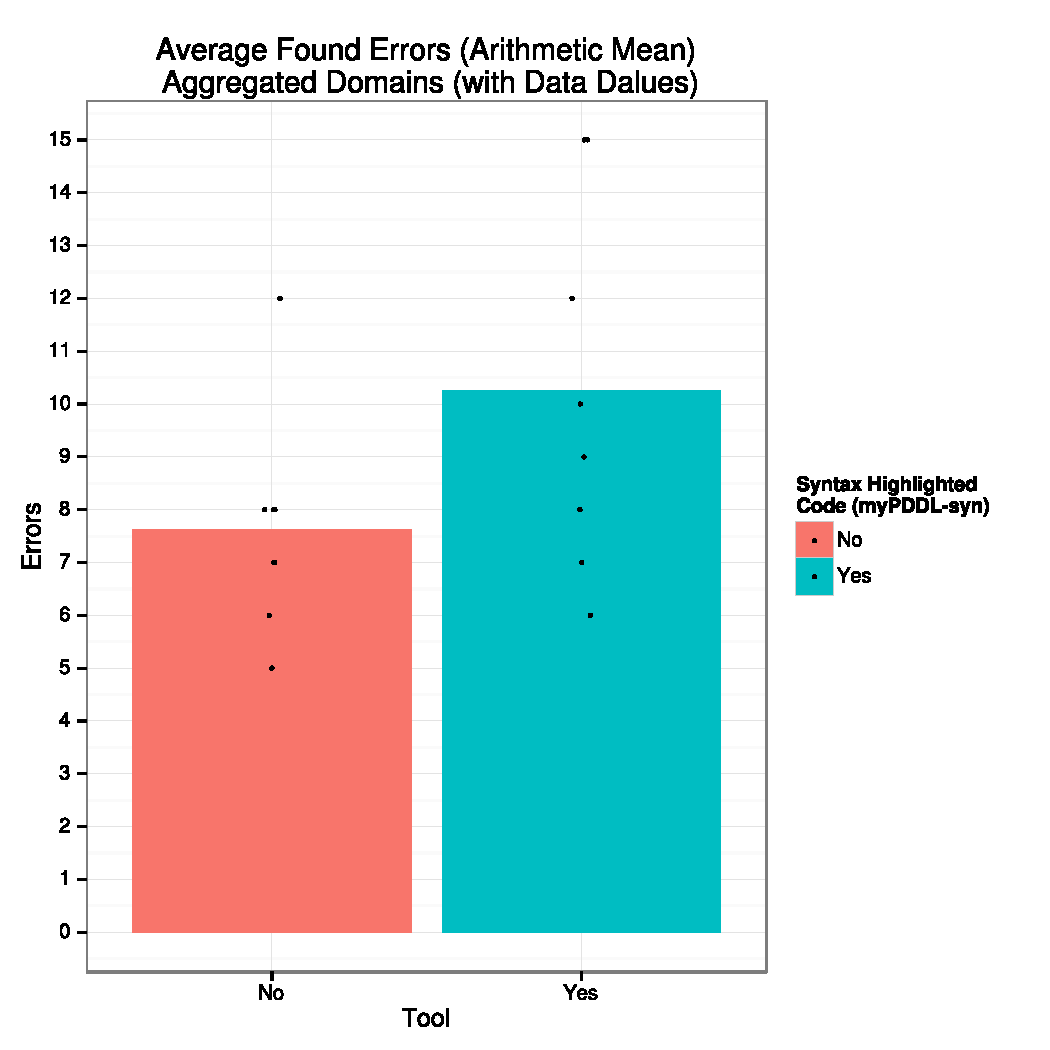
\includegraphics[width=0.7\textwidth]{found-combined.pdf}
\caption{Comparison of detected errors with and without
the syntax highlighting feature. Each cross (\times) shows
the data value of one participant. The bars display the arithmetic
mean.}
\end{figure}

Here, it is worth looking at the raw data, though, and more
specifically the raw data in combination with the comments and remarks
made by the participants during testing. Two participants
(participants 5 and 6) remarked that the syntax highlighting colors
confused them and that they found them more distracting than helpful.
One of them even mentioned that the contrast of the colors used was so
low that they were hard for her to distinguish. She found the same
number of errors with and without syntax highlighting, the other of
the two was the only participant that found less errors with syntax
highlighting than without it. Excluding these two participants from
the analysis results in 49~\% more errors being found with the help
of syntax highlighting. Since only eight participants took part in the
study, splitting the data up further (to compare, for example, the
errors found per domain) did not appear sensible as aggregated data
values would then consist of data from four participants at the most.
A between groups comparison with only four individuals per group is
most likely not going to provide insightful and reliable results
(TODO: source).
\item Type Hierarchy Tasks
\label{sec-5-2-4-2}

Diagram \texttt{fig:task-completions-agg} shows the geometric mean \footnote{The geometric mean is a more accurate measure of the mean for
small sample sizes as task times have a strong tendency to be positively
skewed \cite{sauro2012quantifying}.} of
the task completion time \footnote{The task completion time only includes task times of users who
completed the task successfully.} for each question with and without
the type diagram generator.

\begin{figure}
  \centering
  \hspace{0.5cm}
  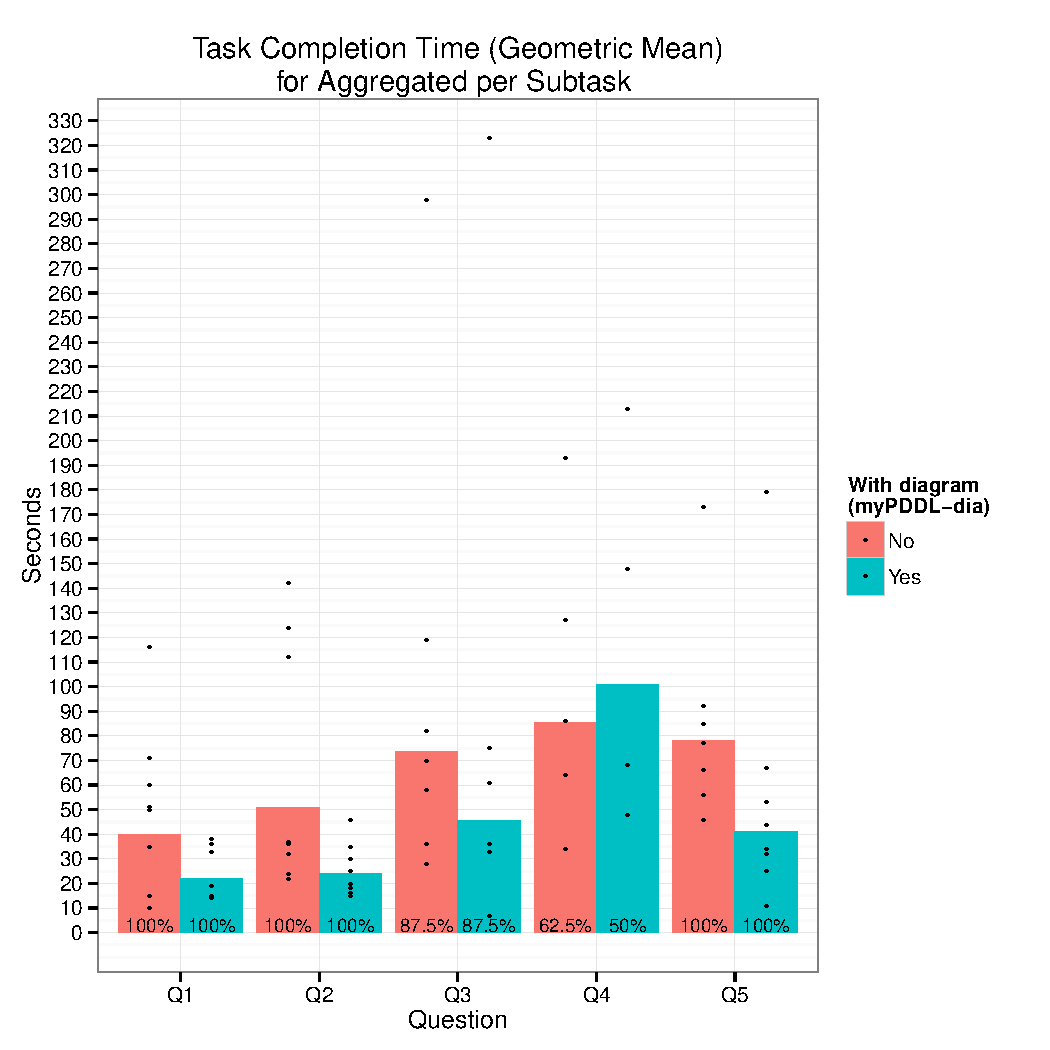
\includegraphics[width=0.7\textwidth]{task-completions-agg.pdf}
  \caption{The diagram shows the geometric mean of the task completion time. The crosses (\times) represent one participant.}
  \label{fig:task-completions-agg}
\end{figure}

It can be seen that when having the type diagram generator available,
participants answer all questions, except question 4, nearly twice as
fast. The fact that the availability of tools did not have a positive
effect on task completion times for question 4 can probably be
attributed to the complexity of this question. In contrast to the
other four questions, to answer question 4 correctly, the participants
were required to look at the actions in the domain file in addition to
the type diagram. Most participants were confused by this, because
they had assumed that once having the type diagram available, it alone
would suffice to answer all questions. This initial confusion cost
some time, thus negatively influencing the time on task.
Therefore, question four is excluded from Diagram
\texttt{task-completions-agg-without-q4}.

\begin{figure}
  \centering
  \includegraphics[width=0.7\textwidth]{ttot1.pdf}
  \caption{Geometric mean of the total time on task without Question 4}
  \label{fig:task-completions-agg-without-q4}
\end{figure}


Diagram \texttt{task-completions-agg-without-q4} illustrates the effect that
the tool availability had on the total time participants spent on a
task, without question 4. It only takes 52\% of the time without tools
to answer questions 1, 2, 3 and 5 once tools can be used.
\item System Usability Scale
\label{sec-5-2-4-3}

\mypddl reached a score of 89.6 on the system usability scale \footnote{The range of possible values for the system usability scale is
0 to 100.},
with a standard deviation of 3.9. Figure \texttt{fig:sus} displays this score
and the data values of the seven participants who completed this
questionnaire. Since the overall mean score of the system usability
scale is approximately 68 with a standard deviation of 12.5
\cite{sauro2011practical}, the score of \mypddl is well above average
with a small standard deviation. A score of 89.6 is usually assigned
to superior products \cite{bangor2008empirical}. Furthermore, 89.6
corresponds approximately to a percentile rank of 99.8 \%, meaning that
it has a better perceived ease-of-use than 99.8 \% of the products in
the database used in \textcite{sauro2011practical}.

\begin{figure}[]
  \centering
  \includegraphics[width=0.7\textwidth]{sus1.pdf}
  \caption{\mypddl got a score of 89.6 on the system usability scale
    that ranges from 0 - 100. Every cross (\times) indicates the
    system usability scale value of one participant. It is evident
    that all scores range in the high end of the scale.}
  \label{fig:sus}
\end{figure}
\end{enumerate}

\subsection{Discussion}
\label{sec-5-2-5}

Although participants’ responses in the System Usability Scale seem to
indicate that myPDDL is an enjoyable software with a high usability,
it is still necessary that it is evaluated with regard to the afore
mentioned criteria in order to reach an informed conclusion concerning
its quality.

\begin{enumerate}
\item Functional Suitability
\label{sec-5-2-5-1}

When comparing the feature diversity of \mypddl with that of other
tools for the same purpose, it becomes immediately evident that
\mypddl is not only up to par, but, integrated into Sublime Text, it
provides a rich developing environment for \pddl files. One of its
strengths lies in being up-to-date and supporting the most recent
\pddl version. Due to the Sublime Text integration, it also offers all
basic editor features and a high customizability. Being the only one
of the four tools capable of visualizing parts of the \pddl code, it
must be understood as complementary to \itsimple, which takes the
opposite approach of transforming \textsc{uml} diagrams into \pddl
files. The fact that \mypddl does not check for semantic errors is not
actually a drawback, as planners will usually detect semantic errors.
All in all, \mypddl combines the most useful tools of \pddlstudio,
\itsimple and \pddlmode for Emacs and strives to support the knowledge
engineer during all phases of the modeling process. Additionally, it
features some unique tools, which have, in part, already been proven
to be helpful in the user study. It can therefore be concluded that
\mypddl provides an appropriate set of functions for developing \pddl
files and is thus functionally suitable.
\item Collaboration
\label{sec-5-2-5-2}

With the growing importance of team work and team members not
necessarily working in the same building or in the same country for
that matter, there is an increasing need for tools supporting the
collaboration effort. In developing \mypddl, this need was sought to
be met by \mypddl-dia. Complex type hierarchies can be hard to
overlook, especially if they were constructed by someone else.
Therefore, a good way of tackling this problem seemed to be by
providing a means to visualize such hierarchies in the form of type
diagrams. But is this really able to help knowledge engineers? This
was tested in the user study by having participants answer questions
on complex type hierarchies that they had never seen before, made up
entirely of non-words (to eliminate the interference of world
knowledge). With the help of the diagram participants were able to
answer questions correctly nearly twice as fast as without this
service. This indicates that \mypddl-gen helps to understand foreign
domain structures faster and more easily, therefore facilitating the
collaboration between knowledge engineers.
\item Experience
\label{sec-5-2-5-3}

Although it is assumed that most people interested in using \mypddl
have some experience in planning, unversed users should not be put off
by a complex or incomprehensible interface. To test if \mypddl is
usable even for novices, it was chosen to only allow for inexperienced
participants in the user study. However they were all required to be
familiar with at least one Lisp dialect because \pddl is Lisp-based.
As described above, participants were asked to watch a 30-minute
interactive planning and \pddl video tutorial, establishing the
basics. Before having to use the \mypddl tools, another three minute
video tutorial introduced \mypddl-syn and \mypddl-dia. None of the
users seemed to have any problems in comprehending either of these
tools after seeing the tutorial. Therefore, it can be concluded that a
small time investment for inexperienced users, and an possibly even
smaller investment for \pddl experts, results in proficient usage of
\mypddl. Nonetheless, two subjects reported having trouble with
\mypddl-syn, because they did not find it helpful or because they
found the colors hard to distinguish. It seems, though, that this
cannot be accounted to inexperience so much as to personal preference.
\item Debugging
\label{sec-5-2-5-4}

To help users find errors faster, the syntax highlighting feature
\mypddl-syn was created. It highlights all syntactically correct
constructs and leaves all syntactical errors non-highlighted. In order
to assess if \mypddl helps in debugging, \mypddl-syn was included in
the usability test. Users were asked to find as many errors as they
could in a specified amount of time. Six of the eight subjects found
more errors with syntax highlighting than without it, one person found
the same number and one actually found one error less with the tool
available. These latter two users reported being distracted by the
colors. Syntax highlighting is optional in the Sublime Text
integration, thanks to the high customizability, and what is more,
different color schemes allow for the individualization of
\mypddl-syn. However, this option was not made available in the user
study, as it would have been an additional, possibly confounding
variable, making the results harder to interpret. While eight people
seem too few to generalize the numbers, it can be said that \mypddl
with \mypddl-syn seems to help the majority of users in debugging.

\item Maintenance
\label{sec-5-2-5-5}

The possibility to maintain \pddl files is a key aspect of \mypddl.
The automatically generated type diagram (\mypddl-dia) gives an
overview of the domain structure, and thereby serves as a continuous
means of documentation. In addition, the diagram supports the
understanding of existing or extended domains provided by other
knowledge engineers. Helping to understand foreign code, though, it
follows logically that \mypddl-dia also helps in coming back and
changing one’s own models if some time has elapsed since they were
last edited. The basic revision control feature of \mypddl-dia keeps
track of changes, making it easy to revert to a previous domain
version. Furthermore, \mypddl-new encourages adhering to an organized
project structure and stores corresponding files at the same location.
Text-based modeling facilitates using a common revision control system
like Git \cite{gronniger2007textbased}. The automatically created
readme file can induce the user to provide further information and
documentation about the \pddl project. When using a web-based hosting
service, the readme file is usually prominently displayed on the home
page of the project.

\item Efficiency
\label{sec-5-2-5-6}

All \mypddl tools are intended to increase the efficiency with which
\pddl files are made. For one, code snippets enable the fast creation
of large and correct code skeletons that only still need to be filled
in. While the type diagram generator facilitates collaboration, it can
also be used to double check if the type hierarchy and the predicates
that use the types have been implemented as intended. Syntax
highlighting can reduce the time spent on searching errors. Code
folding allows users to hide currently irrelevant parts of the code
and automatic indentation increases its legibility. To easily keep
track of all the parts of a project, folders are automatically created
and named. Lastly, it is also possible to customize \mypddl so as to
adapt its look and feel to other programs one is already familiar
with, or simply to make it more enjoyable to use. All these features
should increase the efficiency, and especially skilled knowledge
engineers should be able to produce acceptable models very quickly
with the help of \mypddl.
\item Support
\label{sec-5-2-5-7}

\mypddl can be installed using Sublime Text's Package Control
\cite{stpackage}. This allows for an easy installation and staying
up-to-date with future versions. In order to provide global access and
with it the possibility for developing an active community, the
project source code is hosted on GitHub \footnote{\url{https://github.com/Pold87/myPDDL}}. An additional project
site \footnote{\url{http://pold87.github.io/sublime-pddl/}} provides \mypddl video introductions, a manual and room
for discussing features and reporting bugs.


  \begin{figure}
    \centering
    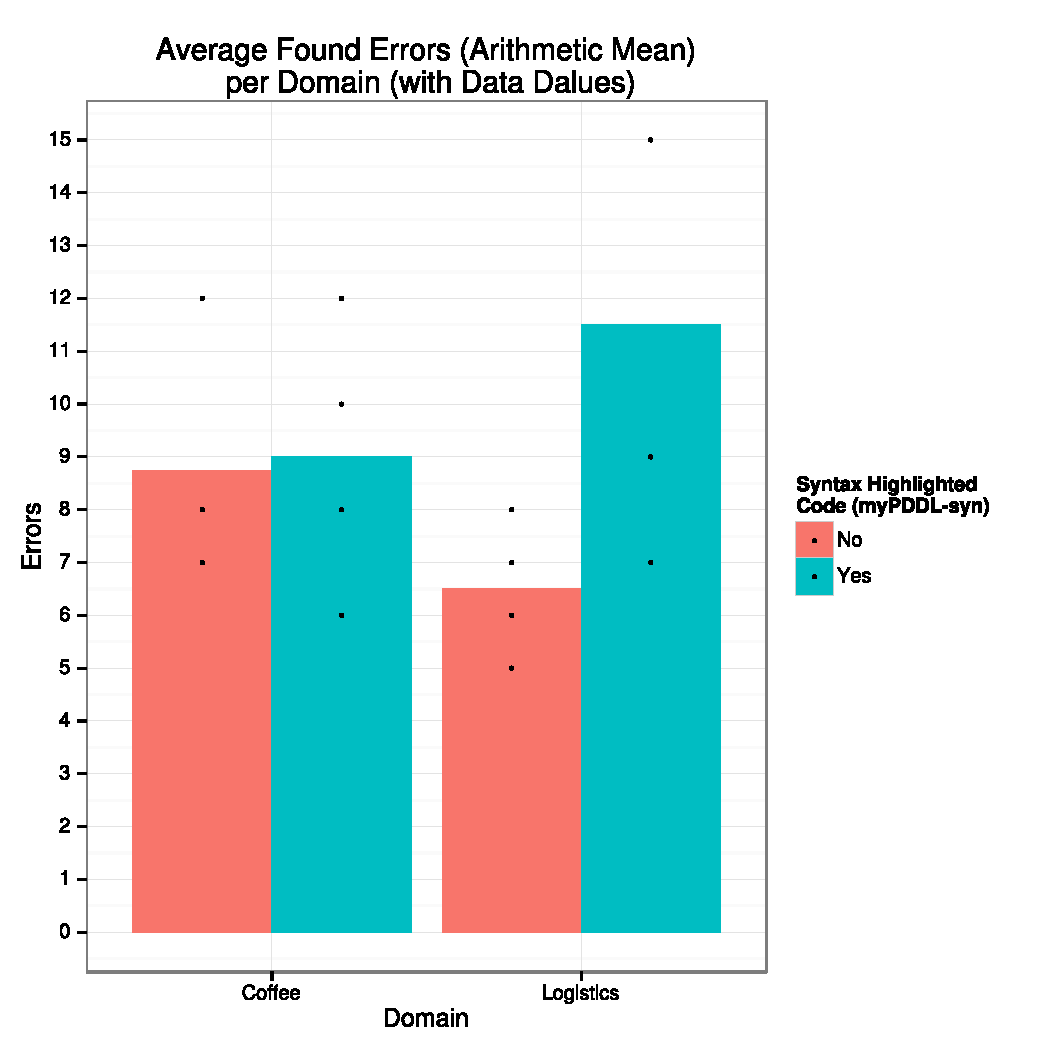
\includegraphics[width=0.8\textwidth]{found-errors-splitted.pdf}
\caption[]{\label{fig:planet-splisus}The Domain Planet Splisus.}
  \end{figure}
\end{enumerate}
\chapter{Conclusion and Future Work}
\label{sec-6}
\label{ch:conclusion}

\mypddl has been designed to support knowledge engineers in modeling
planning task specifications as well as in understanding, modifying,
extending and using existing planning domains. \mypddl is written in a
modular fashion, is extensible and customizable.
Implemented features comprise code editing features, namely syntax
highlighting and code snippets, a type diagram generator and a
distance calculator.

The user study shows some initial evidence that the core features,
syntax highlighting (\mypddl-sub) and type diagram generation
(\mypddl-dia) can support knowledge engineers in the design and
analysis process, in particular in error detection and in keeping
track of the domain structure, the type hierarchy and understandingq
predicates using these types.

Knowledge engineers can customize and extend Sublime Text and use
existing text editor features. Although \mypddl is made available in
Sublime Text, users could transfer the ideas to other text editors.

Furthermore the \pddl/Clojure interface can be used to extract
knowledge, specified in another formal language and create \pddl files
from them.

The plug-in for the editor ST could be further extended to provide
features of common integrated developing environments (IDE). A build
script for providing input to a planner for auto-matching domain and
matching problem(s) (or problem and matching domain) in ST could be
convenient.

Detecting semantic errors besides syntactic errors \textcite[as
implemented in][for \textsc{pddl1.2}]\{plch2012inspect\} Studio could be
the next step to detecting errors fast and accurate. Possible semantic
errors could be undeclared variables or predicates in a domain
specification.

Another alternative is to make use of an external helper and, instead
of calculating every entry of the distance matrix. the distance only
if needed, incorporate every possible combination of two locations.

The yearly workshop Knowledge Engineering for Planning and Scheduling
(KEPS) will promote the research in planning and scheduling
technology. Potentially, the main effort of for implementing models in
planning will be shifted from the manual knowledge engineering to the
automated knowledge acquisition (KA). Perception systems,
Nevertheless, a engineer who double-checks the generated tasks will be
irreplaceable.

The PDDL/Clojure interface provides a basis for dynamic and
interactive planning scenarios. So, time-dependent knowledge could be
modeled by adding facts (learning) to and retracting facts (forget)
from facts a \pddl file.

A faster understanding of the domain structure could be beneficial for
the maintenance and application of existing domains and problems, and,
possibly for the communication between engineers. Finally, real world
usage of PDDL can be promoted so that the focus of artificial
intelligence planning can also be shifted towards the design of plans,
following the citation "Plans are worthless, but planning is
everything".


\printbibheading
\printbibliography[nottype=online,heading=subbibliography,title=Paper Sources]
\printbibliography[type=online (\, heading=subbibliography) (\, title=Website) Sources]

\chapter{Appendix}
\label{sec-7}


\section{General}
\label{sec-7-1}
\begin{listing}[H]
\begin{minted}[fontsize=\small,bgcolor=dhscodebg,rulecolor=\color{gray!40},frame=lines,framesep=5\fboxrule,framerule=1pt,tabsize=2]{text}
; Hacker World - A realistic example
(define (domain hacker-world)
        (:requirements :typing
                       :negative-preconditions
                       :fluents)

  (:types hacker non-hacker - person
          desk chair - furniture
          laptop workstation - computer
          pizza burgers fries - food
          pepperoni supreme - pizza
          computer food person furniture software - object
          number)

    (:predicates (has ?s - software ?p - person)
                 (hungry ?p - person)
                 (vulnerable ?s - software)
                 (exploited ?s - software)
                 (distance ?o1 ?o2 - object ?x - number)
                 (location ?o - object ?x ?y - number))

;; Eat a delicious pizza
  (:action eat-pizza
    :parameters (?pi - pizza ?p - person)
    :precondition (and (hungry ?p)
                       (has ?pi ?p))
    :effect (and (not (hungry ?p))
                 (not (has ?pi ?p))))

 ;; Exploit vulnerable software of a victim
  (:action exploit        
    :parameters (?h - hacker ?s - software ?p - person)
    :precondition (and (has ?s ?p)
                       (vulnerable ?s)
                       (not (hungry ?h)))
    :effect (exploited ?s))

 ;; Move a piece of furniture
  (:action move
    :parameters (?f - furniture ?old-x ?old-y ?new-x ?new-y)
    :effect (and (location ?f ?new-x ?new-y)
                 (not (location ?f ?old-x ?old-y)))))
\end{minted}
\caption{Hacker World}
\end{listing}

\begin{listing}[H]
\begin{minted}[fontsize=\small,bgcolor=dhscodebg,rulecolor=\color{gray!40},frame=lines,framesep=5\fboxrule,framerule=1pt,tabsize=2]{text}
(define (problem garys-huge-problem)

        (:domain hacker-world)

        (:objects big-pepperoni - pepperoni
                gary - hacker
                gisela - non-hacker
                magicfailureapp - software)

        (:init (hungry gary)
                   (has big-pepperoni gary)
                   (vulnerable magicfailureapp)
                   (has magicfailureapp gisela))

        (:goal (exploited magicfailureapp)))
\end{minted}
\caption{Garys' Huge Problem}
\end{listing}
\section{Usability Test}
\label{sec-7-2}
\subsection{Design}
\label{sec-7-2-1}


\begin{table}[htb]
\centering
\begin{tabular}{l|llll}
\textbf{S} & \textbf{Order} &  &  & \\
\hline
A & \emph{Planet Splisus} & \emph{Logistics} & Store & Coffee\\
B & Store & Coffee & \emph{Planet Splisus} & \emph{Logistics}\\
C & Planet Splisus & Logistics & \emph{Store} & \emph{Coffee}\\
D & \emph{Store} & \emph{Coffee} & Planet Splisus & Logistics\\
E & \emph{Logistics} & \emph{Planet Splisus} & Coffee & Store\\
F & Coffee & Store & \emph{Logistics} & \emph{Planet Splisus}\\
G & Logistics & Planet Splisus & \emph{Coffee} & \emph{Store}\\
H & \emph{Coffee} & \emph{Store} & Logistics & Planet Splisus\\
\end{tabular}\caption{\label{tab:order}The order of tasks in the experiment}

\end{table}

\emph{Italic}: Tools part

\begin{table}[htb]
\centering
\begin{tabular}{lrr}
\textbf{Fehlertyp} & \textbf{Logistics} & \textbf{Coffee}\\
Extra Zeichen & 4 & 4\\
Fehlendes Zeichen & 3 & 3\\
Tippfehler & 2 & 2\\
Wortverwechslung & 2 & 2\\
Zeichenvertauschung & 2 & 2\\
Zusatz & 1 & 1\\
Variablenfehler & 1 & 1\\
Klammerfehler & 1 & 1\\
Fehlende Syntax & 1 & 1\\
\hline
Gesamt & 17 & 17\\
\end{tabular}\caption{\label{tab:errors}The errors in the domains \emph{Logistics} and \emph{Coffee}}

\end{table}
\section{Fragen}
\label{sec-7-3}
\chapter{Lösung - Planet Splisus}
\label{sec-8}

\begin{enumerate}
\item Ja, \texttt{Flipsis} sind \texttt{Splis}, \texttt{Splis} sind \texttt{Gids} und \texttt{Gids} sind \texttt{Ruffisplisus}.
\item Nein, \texttt{Schloks} sind keine \texttt{Splis}.
\item Nein, \texttt{Merle} sind \texttt{Splis} aber keine \texttt{Splus}.
\item Nein, \texttt{Spleus} sind zwar \texttt{Splos} und \texttt{Hurpf} sind \texttt{Splis}, weshalb
\texttt{Spleus} und \texttt{Hurpf} verheiratet (\texttt{married}) sein könnten,
aber \texttt{Hurpf} sind keine \texttt{Sipsi} und nur \texttt{Sipsi} können
Waffen (\texttt{has-weapon ?h - sipsi)} besitzen. Laut der Aktion \texttt{kill}
muss man zum Umbringen eine Waffe besitzen.
\item \begin{itemize}
\item \texttt{Ruffisplisus} - Wesen
\item \texttt{Lech} - Orte
\item \texttt{Mak} - Nahrung
\end{itemize}
\end{enumerate}
\chapter{Lösung - Store}
\label{sec-9}

\begin{enumerate}
\item Ja, \texttt{Lulas} sind \texttt{Nulls} und \texttt{Nulls} sind \texttt{Minis}.
\item Nein, nur \texttt{Nulls} sind \texttt{Zahls}.
\item Ja, \texttt{Iltre} sind vom Typ \texttt{Lala} (\texttt{Iltre}, \texttt{Nulls}, \texttt{Minis}, \texttt{Lala})
und können an einem Arbeitsplatz (\texttt{workplace}) vom Typ \texttt{Knozi}
arbeiten, da diese wiederum \texttt{Lolas} sein können (\texttt{Lola}, \texttt{Zahls},
\texttt{Knozi})
\item Nein, denn nur ein Objekt vom Typ \texttt{Spax} kann ein Produkt am Ende
eines Verkaufsvorgangs besitzen und \texttt{Kostas} sind keine \texttt{Spax}.
\item \begin{itemize}
\item \texttt{Lala} - Menschen
\item \texttt{Lila} - Produkte
\item \texttt{Lola} - Orte
\end{itemize}
\end{enumerate}
\newpage

\chapter{Fehlerliste - Logistics Domain}
\label{sec-10}
\vspace{0.5cm}
\begin{center}
\begin{tabular}{rrlll}
\# & \textbf{Zeile} & \textbf{Fehler} & \textbf{Korrektur} & \textbf{Fehlertyp}\\
1 & 3 & ?logistics & logistics & extra Zeichen\\
2 & 6 & :types & :typing & Wortverwechslung\\
3 & 8 & :typing & :types & Wortverwechslung\\
4 & 11 & car 2 & car2 & extra Zeichen\\
5 & 16 & = true & Komplett weg & Zusatz\\
6 & 18 & ??veh & ?veh & extra Zeichen\\
7 & 22 & ?tr & ?t & Variablenfehler\\
8 & 24 & incity & in-city & fehlendes Zeichen\\
9 & 31 & n0t & not & Tippfehler\\
10 & 35 & ?to airport & ?to – aiport & fehlendes Zeichen\\
11 & 42 & parameters: & :parameters & Zeichenvertauschung\\
12 & 43 & precondition: & :precondition & Zeichenvertauschung\\
13 & 37 & ay & at & Tippfehler\\
14 & 45 & ) & Klammer entfernen & Klammerfehler\\
15 & 49 & p & ?p & fehlendes Zeichen\\
16 & 51 & ?p ?v & (at ?p ?v) & fehlende Syntax\\
17 & 54 & ?p - ?l & ?p ?l & extra Zeichen\\
\end{tabular}
\end{center}

\newpage

\chapter{Fehlerliste - Coffee Domain}
\label{sec-11}
\vspace{0.5cm}
\begin{center}
\begin{tabular}{rrlll}
\# & \textbf{Zeile} & \textbf{Fehler} & \textbf{Korrektur} & \textbf{Fehlertypen}\\
1 & 3 & COFFEE & (domain COFFEE) & fehlende Syntax\\
2 & 6 & requirements & :requirements & fehlendes Zeichen\\
3 & 9 & \_ & - & Zeichenvertauschung\\
4 & 10 & (at ?l – location) & location & Zusatz\\
5 & 11 & ?coffee & coffee & extra Zeichen\\
6 & 20 & \$k & ?k & Zeichenvertauschung\\
7 & 21 & :preconditions & :precondition & Wortverwechslung\\
8 & 25 & \_furniture & furniture & extra Zeichen\\
9 & 27 & ?fu & ?f & Variablenfehler\\
10 & 32 & :parameters: & :parameters & extra Zeichen\\
11 & 33 & änd & and & Tippfehler\\
12 & 36 & location & location wurde nicht definiert & Wortverwechselung\\
13 & 42 & ?fromr & ?from-r & fehlendes Zeichen\\
14 & 44 & ?tor & ?to-r & fehlendes Zeichen\\
15 & 47 & cjp & cup & Tippfehler\\
16 & 52 & ?hand-over & hand-over & extra Zeichen\\
17 & 55 & Klammer zu viel & Klammer entfernen & Klammerfehler\\
\end{tabular}
\end{center}

\newpage

\chapter{Fehleranalyse}
\label{sec-12}
\vspace{0.5cm}
\begin{center}
\begin{tabular}{lrr}
\textbf{Fehlertyp} & \textbf{Logistics} & \textbf{Coffee}\\
Extra Zeichen & 4 & 4\\
Fehlendes Zeichen & 3 & 3\\
Tippfehler & 2 & 2\\
Wortverwechslung & 2 & 2\\
Zeichenvertauschung & 2 & 2\\
Zusatz & 1 & 1\\
Variablenfehler & 1 & 1\\
Klammerfehler & 1 & 1\\
Fehlende Syntax & 1 & 1\\
\hline
Gesamt & 17 & 17\\
\end{tabular}
\end{center}


\newpage
\chapter{Coffee Domain}
\label{sec-13}
\begin{verbatim}
;;;; Coffee Domain

(define COFFEE

  (requirements
    :typing)

  (:types room - location
          robot human _ agent
          furniture door - (at ?l - location)
          kettle ?coffee cup water - movable
          location agent movable - object)

  (:predicates (at ?l - location ?o - object)
               (have ?m - movable ?a - agent)
               (hot ?m - movable)
               (on ?f - furniture ?m - movable))

  (:action boil
    :parameters (?m - movable $k - kettle ?a - agent)
    :preconditions (have ?m ?a)
    :effect (hot ?m))

  (:action grip-some
    :parameters (?m - movable ?r - robot ?f - _furniture ?l - location)
    :precondition (and (at ?l ?r)
                       (on ?fu ?m)
                       (at ?l ?f))
    :effect (and (have ?m ?r)))

  (:action move
    :parameters: (?m - movable ?a - agent ?from ?to - location)
    :precondition (or (änd (at ?from ?a)
                           (at ?from ?m))
                      (and (at ?from ?m)
                           (location ?from ?a)))
    :effect (and (not (at ?from ?m))
                 (at ?to ?m)))

  (:action change-room
    :parameters (?from-r ?to-r - room ?a - agent)
    :precondition (at ?fromr ?a) 
    :effect (and (not (at ?from-r ?a))
                 (at ?tor ?a)))

  (:action prep-coffee
    :parameters (?a - agent ?c - cjp ?w - water ?cof - coffee)
    :precondition (and (have ?c ?a)
                       (hot ?w))
    :effect (have ?cof ?a))

  (:action ?hand-over
    :parameters (?m - movable ?a1 - agent ?a2 - agent)
    :precondition (have ?m ?a1))
    :effect (and (not (have ?m ?a1))
                 (have ?m ?a2))))
\end{verbatim}

\newpage

\chapter{Logistics Domain}
\label{sec-14}
\begin{verbatim}
;;;; Logistics domain

(define (domain ?logistics)

  (:requirements
    :types) 

  (:typing truck airplane motorboat - vehicle
           package vehicle suitcase furniture - thing
           airport garage station - location
           car1 car 2 car3 - vehicle
           city location thing - object)

  (:predicates (in-city ?l - location ?c - city)
               (at ?obj - thing ?l - location)
               (key ?v - vehicle) = true
               (full ?v - vehicle)
               (in ?p - package ??veh - vehicle))

  (:action drive
    :parameters (?t - truck ?from ?to - location ?c - city)
    :precondition (and (at ?tr ?from)
                       (in-city ?from ?c)
                       (incity ?to ?c))
    :effect (and (not (at ?t ?from))
                 (at ?t ?to)))

  (:action fly
    :parameters (?a - airplane ?from ?to - airport)
    :precondition (at ?a ?from)
    :effect (and (n0t (at ?a ?from))
                 (at ?a ?to)))

  (:action fuel
    :parameters (?v - vehicle ?c - city ?to airport)
    :precondition (and (not (full ?v))
                       (in-city ?to ?c)
                       (at ?v ?to))
    :effect (full ?v))                   

  (:action load
    parameters: (?v - vehicle ?p - package ?l - location)
    precondition: (and (?v ?l)
                       (at ?p ?l))
    :effect (and (ay ?p ?l)
                 (in ?p ?v)))

  (:action unload
    :parameters (?v - vehicle p - package ?l - location)
    :precondition (and (at ?v ?l)
                           ?p ?v)
    :effects (and (not (in ?p ?v))
                  (at ?p - ?l))))
\end{verbatim}

\newpage

\chapter{Planet Splisus}
\label{sec-15}
\begin{verbatim}
(define (domain splisus) 

  (:requirements :typing)

  (:types splis - gid
          spleus - splos
          schprok schlok - splus
          rud mekle - lech
          hulpf hurpf - hupf
          sipsi flipsi hupf - splis
          schmok schkok - splus
          gid splos splus - ruffisplisus
          merle - hupf
          ruffisplisus mak lech - object)

  (:predicates (father-of ?r1 - ruffisplisus ?r2 - ruffisplisus)
               (married ?s1 - splos ?s2 - splis)
               (has-weapon ?h - sipsi)
               (dead ?r1 - ruffisplisus)
               (at ?l - lech ?r - ruffisplisus))

  (:action kill
    :parameters (?l - lech ?r1 - ruffisplisus ?s - splis)
    :precondition (and (at ?l ?r1)
                       (at ?l ?s)
                       (married ?r1 ?s)
                       (has-weapon ?s))
    :effect (and (dead ?r1)
            (not (married ?r1 ?s)))))
\end{verbatim}

\newpage

\chapter{Store}
\label{sec-16}
\begin{verbatim}
(define (domain store)

  (:requirements :typing)

  (:types lala lila - zahls
          blisis blusis - ultri
          iltre lula - nulls
          zahls schwinds - knozi
          minis - lala
          ultri sopple schmitzl - lila
          ultres raglos wexis - lola
          kosta - nulls
          nulls spax - minis
          lola - zahls
          knozi schmus - object)

  (:predicates (product ?k - knozi) ; Produkt
               (workplace ?l1 - lola ?l2 - lala) ; Arbeitsplatz einer Person
               (product-at ?l1 - lola ?l2 - lila) ; Ort eines Produkts
               (cashier ?k - knozi) ; Kassierer / Verkäufer
               (customer ?s - spax) ; Kunde
               (owns ?l - lila ?s - spax)) ; Eigentum

  (:action sell
    :parameters (?p - lila ?z - zahls ?l - lola ?w - wexis ?s - spax)
    :precondition (and (product ?p)
                       (cashier ?z)
                       (product-at ?l ?p)
                       (customer ?s))
    :effect (and (product-at ?w ?p)
                 (not (product-at ?l ?p))
                 (owns ?p ?s))))
\end{verbatim}
\section{Code}
\label{sec-16-1}

This code can also be found on the enclosed CD, and on the Internet
page \url{https://github.com/pold87/sublime-pddl} (most recent version).

The website \url{http://pold87.github.io/sublime-pddl/} is the accompanying
website for this project.

\begin{minted}[fontsize=\small,bgcolor=dhscodebg,rulecolor=\color{gray!40},frame=lines,framesep=5\fboxrule,framerule=1pt,tabsize=2]{clojure}
(ns org-ba.core
  (:gen-class :main true)
  (:require [clojure.tools.reader.edn :as edn]
            [clojure.java.io :as io]
            [clojure.pprint :as pprint]
            [dorothy.core :as doro]
            [rhizome.viz :as rhi]
            [clojure.math.numeric-tower :as math]
            [quil.core :as quil]
            [clojure.java.shell :as shell]
            [me.raynes.conch :as conch]
            [me.raynes.conch.low-level :as conch-sh]
            [fipp.printer :as p]
            [fipp.edn :refer (pprint) :rename {pprint fipp}]
            [me.raynes.fs :as fs])
  (:import [javax.swing JPanel JButton JFrame JLabel]
           [java.awt.image BufferedImage BufferedImageOp]
           [java.io File]))
\end{minted}

\begin{minted}[fontsize=\small,bgcolor=dhscodebg,rulecolor=\color{gray!40},frame=lines,framesep=5\fboxrule,framerule=1pt,tabsize=2]{clojure}
(defn read-lispstyle-edn
  "Read one s-expression from a file"
  [filename]
  (with-open [rdr (java.io.PushbackReader. (clojure.java.io/reader filename))]
    (edn/read rdr)))
\end{minted}

\begin{minted}[fontsize=\small,bgcolor=dhscodebg,rulecolor=\color{gray!40},frame=lines,framesep=5\fboxrule,framerule=1pt,tabsize=2]{clojure}
(defmacro write->file
  "Writes body to the given file name"
  [filename & body]
  `(do
     (with-open [w# (io/writer ~filename)]
     (binding [*out* w#]
       ~@body))
  (println "Written to file: " ~filename)))
\end{minted}

\begin{minted}[fontsize=\small,bgcolor=dhscodebg,rulecolor=\color{gray!40},frame=lines,framesep=5\fboxrule,framerule=1pt,tabsize=2]{clojure}
(defn read-objs
  "Read \textsc{pddl} objects from a file and add type
  (e.g. 'table bed' -> (list table - furniture
                        bed - furniture))"
  [file object-type]
  (as-> (slurp file) objs
        (clojure.string/split objs #"\s")
        (map #(str % " - " object-type) objs)))
\end{minted}



\begin{minted}[fontsize=\small,bgcolor=dhscodebg,rulecolor=\color{gray!40},frame=lines,framesep=5\fboxrule,framerule=1pt,tabsize=2]{clojure}
(defn create-pddl
  "Creates a \textsc{pddl} file from a list of objects and locations"
  [objs-file objs-type]
  (str
   "(define (domain domainName)

  (:requirements
     :durative-actions
     :equality
     :negative-preconditions
     :numeric-fluents
     :object-fluents
     :typing)

  (:types\n"
   (pprint/cl-format nil "~{~&~5@T~a~}" (read-objs objs-file objs-type))
   ")

  (:constants

  )

  (:predicates

  )

  (:functions

  )

  (:durative-action actionName
     :parameters (?x - <objectType>)
     :duration (= ?duration #duration)
     :condition (at start <effects>)
     :effect (at end <effects>))
)"
   ))
\end{minted}


\begin{minted}[fontsize=\small,bgcolor=dhscodebg,rulecolor=\color{gray!40},frame=lines,framesep=5\fboxrule,framerule=1pt,tabsize=2]{clojure}
(defn split-up
  "Split a \textsc{pddl} type list (:types obj1.1 obj1.2 - objT1 obj2 - objT2 ...)
  into strings of subtypes and associated types,
  [[subytype1 subtype 2 ... - type][subtype1 subtype2 ...][type]"
  [coll]
  ;; Remove ':types' if it is present.
  (let [coll (if (= :types (first coll))
               (rest coll)
               coll)]
    ;; Capturing group 1 is type1.1 type1.2.
    ;; Capturing group 1 is type1.
    (re-seq #"((?:(?:\b[a-zA-Z](?:\w|-|_)+)\s+)+)-\s+(\b[a-zA-Z](?:\w|-|_)+)"
            (clojure.string/join " " coll))))
\end{minted}

\begin{minted}[fontsize=\small,bgcolor=dhscodebg,rulecolor=\color{gray!40},frame=lines,framesep=5\fboxrule,framerule=1pt,tabsize=2]{clojure}
(defn types->hash-map-helper
  "Convert splitted type list (['<expr>' '<subtype1.1> <subtype1.2> ...' '<type1>']
  to a hash-map {'<type1>': ['<subtype1.1>' '<subtype1.2>' ...], '<type2>': ...}"
  [coll]
  (reduce (fn [h-map [_ objs obj-type]]
            (let [key-obj-type (keyword obj-type)
                  existing-vals (key-obj-type h-map)]
              (assoc h-map
                key-obj-type
                (concat existing-vals
                        (clojure.string/split objs #"\s")))))
          {}
          coll))
\end{minted}

\begin{minted}[fontsize=\small,bgcolor=dhscodebg,rulecolor=\color{gray!40},frame=lines,framesep=5\fboxrule,framerule=1pt,tabsize=2]{clojure}
(defn types->hash-map
  "Splits types and converts them into a hash-map"
  [pddl-types]
  (types->hash-map-helper (split-up pddl-types)))
\end{minted}

\begin{minted}[fontsize=\small,bgcolor=dhscodebg,rulecolor=\color{gray!40},frame=lines,framesep=5\fboxrule,framerule=1pt,tabsize=2]{clojure}
(defn map-entry->TikZ-seq
  "Converts a hashmap entry (:key [val1 val2 ...])
to a TikZ string (key -- { val1, val2 })"
  [entry]
  (str
   (name (key entry))
   " -- "
   "{" (clojure.string/join ", " (val entry)) "}"))
\end{minted}

\begin{minted}[fontsize=\small,bgcolor=dhscodebg,rulecolor=\color{gray!40},frame=lines,framesep=5\fboxrule,framerule=1pt,tabsize=2]{clojure}
(defn hash-map->TikZ-out
  "Converts complete \textsc{pddl} type hash-map to TikZ file"
  [h-map]
  (str
   "\\documentclass[tikz]{standalone}

\\usepackage[utf8]{inputenc}

\\usepackage{tikz}

\\usetikzlibrary{graphdrawing}
\\usetikzlibrary{graphs}
\\usegdlibrary{layered,trees}

\\begin{document}

\\begin{tikzpicture}

\\graph[layered layout, nodes={draw,circle,fill=blue!20,font=\\bfseries}]
{
  " (clojure.string/join ",\n  " (map map-entry->TikZ-seq h-map))
  "
};

\\end{tikzpicture}
\\end{document}"))
\end{minted}

\begin{minted}[fontsize=\small,bgcolor=dhscodebg,rulecolor=\color{gray!40},frame=lines,framesep=5\fboxrule,framerule=1pt,tabsize=2]{clojure}
(defn types-map-entry->dot-language
  "Converts one hash-map entry
to the dot language"
  [entry]
  (str
   "\"" (name (key entry)) "\""
   " -> "
   "{" (clojure.string/join " " (map #(str "\"" % "\"")  (val entry))) "}"))
\end{minted}

\begin{minted}[fontsize=\small,bgcolor=dhscodebg,rulecolor=\color{gray!40},frame=lines,framesep=5\fboxrule,framerule=1pt,tabsize=2]{clojure}
(defn types-hash-map->dot-language
  "Converts a \textsc{pddl} types hash-map
to the dot language notation"
  [pddl-types-map]
  (clojure.string/join "\n" (map types-map-entry->dot-language pddl-types-map)))
\end{minted}

\begin{minted}[fontsize=\small,bgcolor=dhscodebg,rulecolor=\color{gray!40},frame=lines,framesep=5\fboxrule,framerule=1pt,tabsize=2]{clojure}
;;; Read \textsc{pddl} predicates and generate UML 'type' diagram
(defn get-types-in-predicate
  "Takes a \textsc{pddl} predicate,
  e.g. '(at ?x - location ?y - object)
  and returns the involved types, e.g.
  '(location object)"
  [pddl-pred]
  (remove
   (fn [s]
     (let [first-char (first (name s))]
       (or (= \- first-char)
           (= \? first-char)))) (rest pddl-pred)))
\end{minted}

\begin{minted}[fontsize=\small,bgcolor=dhscodebg,rulecolor=\color{gray!40},frame=lines,framesep=5\fboxrule,framerule=1pt,tabsize=2]{clojure}
(defn pddl-pred->hash-map-long
  "Takes a \textsc{pddl} predicate, e.g.
  '(at ?x - location ?y - object) and returns a
  hash-map, that assigns the involved types
  to this predicate, e.g.
  {location [(at ?x - location ?y - object)],
   object [(at ?x - location ?y - object)]}"
  [pddl-pred]
  (reduce (fn [h-map pddl-type]
            (assoc h-map
              pddl-type
              (list pddl-pred)))
          {}
          (get-types-in-predicate pddl-pred)))
\end{minted}

\begin{minted}[fontsize=\small,bgcolor=dhscodebg,rulecolor=\color{gray!40},frame=lines,framesep=5\fboxrule,framerule=1pt,tabsize=2]{clojure}
(pddl-pred->hash-map-long '(at ?x - location ?y - object))
\end{minted}

\begin{minted}[fontsize=\small,bgcolor=dhscodebg,rulecolor=\color{gray!40},frame=lines,framesep=5\fboxrule,framerule=1pt,tabsize=2]{clojure}
;;; TODO: Create short version wiht prolog predicate style
;;; e.g. at/2
(defn all-pddl-preds->hash-map-long
  "Takes a list of \textsc{pddl} predicates and
  returns a hash-map of types and the
  assigned predicate"
  [pddl-preds]
  (let [pddl-preds (if (= :predicates (first pddl-preds))
                     (rest pddl-preds)
                     pddl-preds)]
    (apply merge-with concat
           (map pddl-pred->hash-map-long pddl-preds))))
\end{minted}

\begin{minted}[fontsize=\small,bgcolor=dhscodebg,rulecolor=\color{gray!40},frame=lines,framesep=5\fboxrule,framerule=1pt,tabsize=2]{clojure}
(defn hash-map->dot
  "Converts a hash-map to
  dot language for creating
  UML diagrams"
  [h-map]  
  (map (fn [map-entry]
         (str (key map-entry)
              "[label = \"{"
              (key map-entry)
              "|"
              (clojure.string/join "\\l"  (val map-entry))
              "}\"]\n"))
       h-map))
\end{minted}

\begin{minted}[fontsize=\small,bgcolor=dhscodebg,rulecolor=\color{gray!40},frame=lines,framesep=5\fboxrule,framerule=1pt,tabsize=2]{clojure}
(defn hash-map->dot-with-style
  "Adds dot template to
hash-map>dot"
  [h-map]
  (str
   "digraph hierarchy {
node[shape=record,style=filled,fillcolor=gray92]
edge[dir=back, arrowtail=empty]
\n"
   (clojure.string/join (hash-map->dot h-map))
   "}"))
\end{minted}


\begin{minted}[fontsize=\small,bgcolor=dhscodebg,rulecolor=\color{gray!40},frame=lines,framesep=5\fboxrule,framerule=1pt,tabsize=2]{clojure}
(defn \textsc{pddl}->dot-with-style
  "Adds dot template to
hash-map>dot"
  [preds types]
  (str
   "digraph hierarchy {
node[shape=record,style=filled,fillcolor=gray92]
edge[dir=back, arrowtail=empty]
\n"

   (clojure.string/join (hash-map->dot (all-pddl-preds->hash-map-long preds)))
   (types-hash-map->dot-language (types->hash-map types))

   "}"))
\end{minted}

\begin{minted}[fontsize=\small,bgcolor=dhscodebg,rulecolor=\color{gray!40},frame=lines,framesep=5\fboxrule,framerule=1pt,tabsize=2]{clojure}
(defn get-\textsc{pddl}-construct
  "Takes a \textsc{pddl} keyword and a \textsc{pddl} domain/problem
file and returns all parts of the file that
belong to the \textsc{pddl} keyword."
  [pddl-keyword pddl-file]
  (filter #(and (seq? %)
                (= (keyword pddl-keyword)
                   (first %)))
          (read-lispstyle-edn pddl-file)))
\end{minted}

\begin{minted}[fontsize=\small,bgcolor=dhscodebg,rulecolor=\color{gray!40},frame=lines,framesep=5\fboxrule,framerule=1pt,tabsize=2]{clojure}
; TODO: Throw error if length != 1
(defn get-\textsc{pddl}-predicates
  "Get all predicates in a \textsc{pddl} file"
  [pddl-file]
  (first (get-\textsc{pddl}-construct 'predicates pddl-file)))

(defn get-\textsc{pddl}-init
  "Get all predicates in a \textsc{pddl} file"
  [pddl-file]
  (first (get-\textsc{pddl}-construct 'init pddl-file)))
\end{minted}


\begin{minted}[fontsize=\small,bgcolor=dhscodebg,rulecolor=\color{gray!40},frame=lines,framesep=5\fboxrule,framerule=1pt,tabsize=2]{clojure}
; TODO: Throw error if length != 1
(defn get-\textsc{pddl}-types
  "Get all types in a \textsc{pddl} file"
  [pddl-file]
  (first (get-\textsc{pddl}-construct 'types pddl-file)))
\end{minted}

\begin{minted}[fontsize=\small,bgcolor=dhscodebg,rulecolor=\color{gray!40},frame=lines,framesep=5\fboxrule,framerule=1pt,tabsize=2]{clojure}
(defn \textsc{pddl}->dot
  "Takes a complete \textsc{pddl} file
and generates a UML type diagram"
  [pddl-file]
  (\textsc{pddl}->dot-with-style (get-\textsc{pddl}-predicates pddl-file)
                        (get-\textsc{pddl}-types pddl-file)))
\end{minted}

\begin{minted}[fontsize=\small,bgcolor=dhscodebg,rulecolor=\color{gray!40},frame=lines,framesep=5\fboxrule,framerule=1pt,tabsize=2]{clojure}
(defn \textsc{pddl}->dot-commandline-input
  "Assumes that the \textsc{pddl} input is
a string and 'reads' this string"
  [pddl-file]
  (print "The type is " (type pddl-file))
  (\textsc{pddl}->dot (edn/read-string pddl-file)))
\end{minted}

\begin{minted}[fontsize=\small,bgcolor=dhscodebg,rulecolor=\color{gray!40},frame=lines,framesep=5\fboxrule,framerule=1pt,tabsize=2]{clojure}
(defn \textsc{pddl}->dot-file-input
  "Reads \textsc{pddl} file"
  [pddl-file-name]
  (\textsc{pddl}->dot pddl-file-name))
\end{minted}

;;;; math helper functions

(defn sqr
  "Square of a number"
  [x]
  (* x x))

(defn round-places [number decimals]
  "Round to decimal places"
  (let [factor (math/expt 10 decimals)]
    (double (/ (math/round (* factor number)) factor))))

(defn euclidean-squared-distance
  "Computes the Euclidean squared distance between two sequences"
  [a b]
  (reduce + (map (comp sqr -) a b)))

(defn euclidean-distance
  "Computes the Euclidean distance between two sequences"
  [a b]
  (math/sqrt (euclidean-squared-distance a b)))

;;;; End math helper functions

(defn calc-distance-good
  "Calculates the distance and writes
the calculated distances to a string
IS VERY GOOD !!!"
  [locations]
  (for [[ \_ loc1 \& xyz-1] locations
        [ \_ loc2 \& xyz-2] locations]
    ;; Euclidean distance rounded to 4 decimal places.
    (list 'distance loc1 loc2 (round-places (euclidean-distance xyz-1 xyz-2) 4))))

(defn get-specified-predicates-in-pddl-file
  "Extracts all locations in the predicates part
(by the specified name) in a \textsc{pddl} file"
  [pddl-file predicate-name]
  (filter \#(and (seq? \%)
                (= predicate-name (first \%)))
          (get-\textsc{pddl}-predicates pddl-file)))

(defn get-specified-inits-in-pddl-file
  "Extracts all locations in the init part
(by the specified name) in a \textsc{pddl} problem"
  [pddl-file predicate-name]
  (filter \#(and (seq? \%)
                (= predicate-name (first \%)))
          (get-\textsc{pddl}-init pddl-file)))

(defn calc-distance
  "Calculate distances of \textsc{pddl} objects"
  [locations]
  (for [[ \_ loc1 \& xyz-1] locations
        [ \_ loc2 \& xyz-2] locations]
    ;; Euclidean distance rounded to 4 decimal places.
    `(\textasciitilde{}'distance \textasciitilde{}loc1 \textasciitilde{}loc2
                 \textasciitilde{}(euclidean-distance xyz-1 xyz-2))))

; LOOK UP: extended equality: 'hello = :hello

(defn add-part-to-\textsc{pddl}
  "Takes a \textsc{pddl} domain or problem
and add the specified part to the
specified position"
  [pddl-file position part]

(map \#(if (and (seq? \%)
               (= (keyword position) (first \%)))
        (concat \% part)
        \%)
     (read-lispstyle-edn pddl-file)))

(defn find-new-file-name
  "Take a filename and determines, the new number
that has to be added to create a new file. E.g.
file1.img file2.img file3.img means that, file4.img
has to be created"
  [filename extension]
  (loop [n 0]
    (if-not (io/.exists (io/as-file
                         (str filename n extension)))
      (str filename n extension)
      (recur (inc n)))))


;;; Copied from \url{https://www.refheap.com/9034}
(defn exit-on-close [sketch]
  "Guarantees that Clojure script will be
exited after the JFrame is closed"
  (let [frame (-> sketch .getParent .getParent .getParent .getParent)]
    (.setDefaultCloseOperation frame javax.swing.JFrame/EXIT\(_{\text{ON}}_{\text{CLOSE}}\))))


(defn extract-locations-from-file
  "Read a Blender \textsc{lisp} file and write object positions to out-file"
  [file-in file-out]
  (let [map-destructorer-local (fn [[\(_{\text{addgv}}\) \_furniture object
                                      [\(_{\text{make}}\)-instance \_object-detail
                                          \_pose [\(_{\text{tfmps}}\)
                                                \_type-name
                                                \_type-num
                                                [\(_{\text{vector}}\)-3d x y z \& more]
                                                \& \_more1]
                                       \& \_more2]]] (list "location" (name object) x y z))]
    (with-open [rdr (java.io.PushbackReader. (io/reader file-in))]
      (println
      (doall
          (map map-destructorer-local
               (filter \#(and (seq? \%) (= 'addgv (first \%)))
                       (take-while \#(not= \% :end)
                                   (repeatedly  \#(edn/read \{:eof :end\} rdr))))))))))


;; Main method
;; TODO: Command line options
(defn -main
  "Runs the input/output scripts"
  [\& args]

(cond
 ;; Create a new \textsc{pddl} project
 (= "new" (first args))
 (let [project-name (second args)]
   (fs/mkdir project-name)
   (fs/mkdir (str project-name "/dot"))
   (fs/mkdir (str project-name "/diagrams"))
   (fs/mkdir (str project-name "/domains"))
   (fs/mkdir (str project-name "/problems"))
   (fs/create (io/file (str project-name "/domain.pddl")))
   (fs/create (io/file (str project-name "/p01.pddl"))))

;; -l flag for adding locations in \textsc{pddl} file
(= (second args) "-l")
(let [content (add-part-to-\textsc{pddl} (first args)
                                'init
                                (calc-distance-good
                                 (get-specified-inits-in-pddl-file (first args)
                                                                   'location)))
      new-filename (clojure.string/replace-first (first args)
                                                 \#"(.+).pddl"
                                                 "\$1-locations.pddl")] ; TODO: location as arg

(write->file new-filename (pprint/pprint content)))


;; Write dot graph to file.
:else
(let [input-domain (first args)
      new-dot-filename (find-new-file-name "dot/dot-diagram" ".dot")
      new-png-filename (find-new-file-name "diagrams/png-diagram" ".png")
      input-domain-filename (fs/name input-domain)
      domain-version (find-new-file-name
                      (str "domains/" input-domain-filename) (fs/extension input-domain))]

;; Save input domain version in folder domains.
(fs/copy+ input-domain domain-version)     

;; Create folders for dot files and png diagrams
(fs/mkdir "dot")
(fs/mkdir "diagrams")

;; Create dot language file in dot folder.
(doall
 (write->file new-dot-filename
              (print (\textsc{pddl}->dot-file-input input-domain))))

;; Create a png file from dot
(fs/exec "dot" "-Tpng" "-o" new-png-filename new-dot-filename)

;; Settings for displaying the generated diagram.
(def img (ref nil))

(defn setup []
  (quil/background 0)
  (dosync (ref-set img (quil/load-image new-png-filename))))

(def img-size
  (with-open [r (java.io.FileInputStream. new-png-filename)]
    (let [image (javax.imageio.ImageIO/read r)
          img-width (.getWidth image)
          img-height (.getHeight image)]
      [img-width img-height])))

(defn draw []
  (quil/image @img 0 0))

;; Display png file in JFrame.
(exit-on-close
 (quil/sketch
:title (str "\textsc{pddl} Type Diagram - " input-domain-filename)
:setup setup
:draw draw
       :size (vec img-size))))))
\#+END\(_{\text{SRC}}\)

\begin{minted}[fontsize=\small,bgcolor=dhscodebg,rulecolor=\color{gray!40},frame=lines,framesep=5\fboxrule,framerule=1pt,tabsize=2]{text}
# [PackageDev] target_format: plist, ext: tmLanguage
---
name: \textsc{pddl}
scopeName: text.pddl
fileTypes: [pddl]
uuid: 2aef09fc-d29e-4efd-bf1a-974598feb7a9

patterns:

#####################
### Customization ###

- include: '#domain'
- include: '#problem'
- include: '#comment'

##################
### Repository ###

repository:


##############################
### General specifications ###
##############################

  built-in-var:
    match: \?duration 
    name: variable.language.pddl

  variable:
    match: '(?:^|\s+)(\?[a-zA-Z](?:\w|-|_)*)'
    # name: variable.other.pddl
    name: keyword.other.pddl # TODO: changeback again to variable.other.pddl
    # this is just a dirty hack for highlighting

  pddl-expr:
    match: '(?:^|\s+)([a-zA-Z](?:\w|-|_)*)(?!:|\?)\b'
    captures:
      '1': {name: string.unquoted.pddl}
    #name: string.unquoted.pddl

  comment:
    comment: "Comments beginning with ';'"
    name: comment.line.semicolon.pddl
    match: ;.*

  number:
    name: constant.numeric.pddl
    match: \b((0(x|X)[0-9a-fA-F]*)|(([0-9]+\.?[0-9]*)|(\.[0-9]+))((e|E)(\+|-)?[0-9]+)?)(L|l|UL|ul|u|U|F|f|ll|LL|ull|ULL)?\b

  keyword:
    name: storage.type.pddl # TODO: UPDATE
    match: :(constraints|metric|length)


######################
### Domain Helpers ###
######################


  function-keyword:
    name: support.function.pddl
    match: (assign|scale-up|scale-down|increase|decrease)


  # TODO
  other-keyword:
    name: support.other.pddl
    comment: "Remove parent or do sth that the paren isn't highlighted"
    match: \b(forall|(at\s+(start|end))|over)\b


  language-constant:
    name: constant.language.pddl
    match: (start|end|all)

  action-keyword:
    name: keyword.operator.pddl
    match: ':(?i:(parameters|vars|precondition|effect))(?!:|\?)\b'

  durative-action-keyword:
    name: keyword.operator.pddl
    match: ':(?i:(parameters|vars|duration|condition|effect))(?!:|\?)\b'



#############################
### Domain specifications ###
#############################

  domain:  
    patterns:
    - comment: "domain definition "
      name: meta.function.pddl
      begin: '\(\s*((?i:define))\b(?!\s+\(problem)'
      beginCaptures:
        '1': {name: storage.type.pddl}
      end: '\)'
      patterns: 
        - include: '#comment'
        - include: '#domain-name-in-define'
        - include: '#requirement'
        - include: '#types'
        - include: '#constants'
        - include: '#predicates'
        - include: '#new-functions'
        - include: '#action'
        - include: '#durative-action'
        - include: '#any-sexpr'


  domain-name-in-define:
    patterns:
      - comment: "Domain name in problem file"
        name: meta.type.pddl # TODO: NAME
        begin: '\(\s*(?i:(domain))\b'
        end: '\)'
        beginCaptures:
          '1': {name: storage.type.pddl}
        patterns:
          - include: '#comment'
          - name: invalid.illegal.pddl
            match: (\s+(?:\w|-)+){2,}
          - include: '#pddl-expr'

  requirement:
    patterns:
      - comment: "Requirement"
        name: meta.type.pddl # TODO: NAME
        begin: '\(\s*(?i:(:requirements))\b'
        beginCaptures:
          '1': {name: storage.type.pddl}
        end: '\)'
        patterns:
        - name: keyword.other.pddl
          match:  :(?i:(strips|typing|negative-preconditions|disjunctive-preconditions|equality|existential-preconditions|universal-preconditions|quantified-preconditions|conditional-effects|fluents|numeric-fluents|object-fluents|adl|durative-actions|duration-inequalities|continuous-effects|derived-predicates|timed-initial-literals|preferences|constraints|action-costs))\b

  types:
    patterns:
      - comment: "Types"
        name: meta.type.pddl # TODO: NAME
        begin: '\(\s*(?i:(:types))\b'
        end: '\)'
        beginCaptures:
          '1': {name: storage.type.pddl}
        patterns:
          - name: meta.keyword.pddl
            captures:
              '1': {name: constant.character.pddl}
              #'1': {name: string.unquoted.pddl}
              '2': {name: entity.name.function.pdd}
            match:  (-)(?:^|\s+)([a-zA-Z](?:\w|-|_)*)
          - include: '#either'
          - include: '#pddl-expr'
          - include: '#any-sexpr'

  constants:
    patterns:
      - comment: "Constants"
        name: meta.type.pddl # TODO: NAME
        begin: '\(\s*(?i:(:constants))\b'
        end: '\)'
        beginCaptures:
          '1': {name: storage.type.pddl}
        patterns:
          - name: meta.keyword.pddl
            captures:
              '1': {name: entity.name.function.pddl}
              #'1': {name: string.unquoted.pddl}
              '2': {name: entity.name.tag.pddl}
            match:  (-)(?:^|\s+)([a-zA-Z](?:\w|-|_)*)
          - include: '#either'
          - include: '#pddl-expr'

  predicate:
    patterns:
      - begin: '\(\s*((?:\w|-)+)'
        end: '\)'
        beginCaptures:
          '1': {name: storage.type.pddl}
        patterns:
          - include: '#variable'
          - name: meta.name.function.pddl
            captures:
              '1': {name: constant.character.pddl}
              '2': {name: entity.name.function.pddl}
            match: (-)(?:^|\s+)([a-zA-Z](?:\w|-|_)*)

  init-predicate:
    patterns:
      - begin: '\(\s*((?:\w|-)+)'
        end: '\)'
        beginCaptures:
          '1': {name: storage.type.pddl}
        patterns:
          - include: '#pddl-expr'
          - include: '#number'
          - include: '#init-predicate-other'

  init-predicate-other:
    patterns:
      - begin: '\(\s*((?:\w|-)+)'
        end: '\)'
        beginCaptures:
          '1': {name: storage.type.pddl}
        patterns:
          - include: '#pddl-expr'
          - include: '#number'
          - include: '#init-predicate'

  applied-predicate-other:
    patterns:
      - begin: '\(\s*((?:\w|-)+)'
        end: '\)'
        beginCaptures:
          '1': {name: storage.type.pddl}
        patterns:
          - include: '#variable'
          - include: '#pddl-expr'
          - include: '#applied-predicate'

  applied-predicate:
    patterns:
      - begin: '\(\s*((?:\w|-)+)'
        end: '\)'
        beginCaptures:
          '1': {name: storage.type.pddl}
        patterns:
          - include: '#variable'
          - include: '#pddl-expr'
          - include: '#applied-predicate-other'


  function:
    patterns:
      - begin: '\(\s*((?:\w|-)+)'
        end: '(\)\s+-\s+((?:\w|-)+))'
        endCaptures:
          '2': {name: storage.type.pddl}
        beginCaptures:
          '1': {name: storage.type.pddl}
        patterns:
          - include: '#variable'
          - name: meta.name.function.pddl
            captures:
              '1': {name: entity.name.function.pddl}
            match: '-\s+((?:\w|-)+)'


  function-with-either:
    patterns:
      - begin: '\((\w+)'
        end: '(\)\s+-\s+((?:\w|-)+))|\)'
        endCaptures:
          '2': {name: storage.type.pddl}
        beginCaptures:
          '1': {name: storage.type.pddl}
        patterns:
          - include: '#variable'
          - name: meta.name.function.pddl
            captures:
              '1': {name: entity.name.function.pddl}
            match: '-\s+((?:\w|-)+)'

  predicates:
    patterns:
      - comment: "Predicates"
        name: meta.type.pddl # TODO: NAME
        begin: '\(\s*(?i:(:predicates))\b'
        end: '\)'
        beginCaptures:
          '1': {name: storage.type.pddl}
        patterns:
          - include: '#predicate'
          - include: '#any-sexpr'


  connected-predicate-other:
    patterns:
      - comment: "Predicates that are connected via and, or, etc."
        #name: string.unquoted.pddl # TODO: NAME
        begin: '\((and|or|eq|neq|not|=|>=|<=|assign|increase|decrease|scale-up|scale-down|forall|exists|imply|when|\+|-|\*|/)\b'
        end: '\)'
        beginCaptures:
          '1': {name: string.unquoted.pddl}
        patterns:
          - include: '#typed-variable-list'
          - include: '#connected-predicate'
          - include: '#applied-predicate'
          - include: '#variable'
          - include: '#pddl-expr'

  connected-predicate:
    patterns:
      - comment: "Predicates that are connected via and, or, etc."
        name: meta.type.pddl # TODO: NAME
        begin: '\((and|or|eq|neq|not|=|>=|<=|assign|increase|decrease|scale-up|scale-down|forall|exists|imply|when|\+|-|\*|/)\b'
        end: '\)'
        beginCaptures:
          '1': {name: string.unquoted.pddl}
        patterns:
          - include: '#typed-variable-list'
          - include: '#connected-predicate-other'
          - include: '#applied-predicate'
          - include: '#variable'
          - include: '#pddl-expr'

# TODO:
  functions:
    patterns:
      - comment: "Functions"
        name: meta.type.pddl # TODO: NAME
        begin: '\(\s*(?i:(:functions))\b'
        end: '\)'
        beginCaptures:
          '1': {name: storage.type.pddl}
        patterns:
          - include: '#function'
          - begin: '\((either)'
            beginCaptures:      
              '1': {name: entity.name.function.pddl}
              '2': {name: storage.type.pddl}
            patterns:
              - include: '#pddl-expr'
            end: '\)'
         #- include: '#function-with-either'

  either:
    patterns:
      - begin: '(-)\s+\((either)'
        beginCaptures:      
          '1': {name: entity.name.function.pddl}
          '2': {name: storage.type.pddl}
        patterns:
          - include: '#pddl-expr'
        end: '\)'

  new-functions:
    patterns:
      - comment: "Functions"
        name: meta.type.pddl # TODO: NAME
        begin: '\(\s*(?i:(:functions))\b'
        end: '\)'
        beginCaptures:
          '1': {name: storage.type.pddl}
        patterns:
          - include: '#either'
          - include: '#predicate'
          - include: '#pddl-expr'

  typed-variable-list:
    patterns:
      - begin: '\((\?((?:\w|-)+))'
        end: '\)'
        beginCaptures:
          '1': {name: keyword.other.pddl}
        patterns:
          - include: '#variable'
          - name: meta.name.function.pddl
            captures:
              '1': {name: constant.character.pddl}
              '2': {name: entity.name.function.pddl}
            match: '(-)(?:^|\s+)([a-zA-Z](?:\w|-|_)*)(?!:|\?)\b'

  precondition:
    patterns:
      - name: entity.name.function.pddl
        begin: ':precondition\s*'
        end: \b

 # any-sexpr:
 #   patterns:
 #     - match: \(.*\)
 #       patterns:
 #         - include: '$self'


  any-sexpr:
    patterns:
      - begin: '\('
        end: '\)'
        patterns:
          - include: '#any-sexpr-other'
          - match:  (?:\s)*

  any-sexpr-other:
    patterns:
      - begin: '\('
        end: '\)'
        patterns:
          - include: '#any-sexpr'
          - match: (?:\s)*

  action:
    patterns:
      - comment: "Action"
        name: meta.type.pddl # TODO: NAME
        begin: '\(\s*(?i:(:action))\b'
        end: '\)'
        beginCaptures:
          '1': {name: storage.type.pddl}
        patterns:
          - include: '#connected-predicate'
          - include: '#applied-predicate'
          - include: '#pddl-expr'
          - include: '#comment'
          - include: '#typed-variable-list'
          - include: '#action-keyword'
          - include: '#built-in-var'
          - include: '#any-sexpr'

  durative-action:
    patterns:
      - comment: "Durative Action"
        name: meta.type.pddl # TODO: NAME
        begin: '\(\s*(?i:(:durative-action))\b'
        end: '\)'
        beginCaptures:
          '1': {name: storage.type.pddl}
        patterns:
          - include: '#connected-predicate'
          - include: '#applied-predicate'
          - include: '#pddl-expr'
          - include: '#comment'
          - include: '#typed-variable-list'
          - include: '#durativ-action-keyword'
          - include: '#built-in-var'
          - include: '#any-sexpr'

#######################
### Problem Helpers ###
#######################

  problem-name-in-define:
    patterns:
      - comment: "Domain name in problem file"
        name: meta.type.pddl # TODO: NAME
        begin: '\(\s*(?i:(problem))\b'
        end: '\)'
        beginCaptures:
          '1': {name: storage.type.pddl}
        patterns:
          - include: '#comment'
          - name: invalid.illegal.pddl
            match: (\s+(?:\w|-)+){2,}
          - include: '#pddl-expr'

  domain-name-in-problem:
    patterns:
      - comment: "Domain name in problem file"
        name: meta.type.pddl # TODO: NAME
        begin: '\(\s*(?i:(:domain))\b'
        end: '\)'
        beginCaptures:
          '1': {name: storage.type.pddl}
        patterns:
          - include: '#comment'
          - name: invalid.illegal.pddl
            match: (\s+(?:\w|-)+){2,}
          - include: '#pddl-expr'

##############################
### Problem specifications ###
##############################


  problem:  
    patterns:
    - comment: "problem definition"
      name: meta.function.pddl
      begin: '\(\s*((?i:define))\b'
      beginCaptures:
        '1': {name: storage.type.function-type.pddl}
      end: '\)' # Paren after the domain/problem name.
      patterns: 
        - include: '#comment'
        - include: '#problem-name-in-define'
        - include: '#domain-name-in-problem'
        - include: '#inits'
        - include: '#objects'
        - include: '#goal'

  objects:
    patterns:
      - comment: "Objects"
        name: meta.type.pddl # TODO: NAME
        begin: '\(\s*(?i:(:objects))\b'
        end: '\)'
        beginCaptures:
          '1': {name: storage.type.pddl}
        patterns:
          - name: meta.keyword.pddl
            captures:
              '1': {name: entity.name.function.pddl}
              #'1': {name: string.unquoted.pddl}
              '2': {name: entity.name.tag.pddl}
            match:  (-)(?:^|\s+)([a-zA-Z](?:\w|-|_)*)
          - include: '#either'
          - include: '#pddl-expr'

  inits:
    patterns:
      - comment: "Initalized predicates"
        name: meta.type.pddl # TODO: NAME
        begin: '\(\s*(?i:(:init))\b'
        end: '\)'
        beginCaptures:
          '1': {name: storage.type.pddl}
        patterns:
          - include: '#init-predicate'
          - include: '#connected-predicate'
          - include: '#any-sexpr'

  goal:
    patterns:
      - comment: "Goal"
        name: meta.type.pddl # TODO: NAME
        begin: '\(\s*(?i:(:goal))\b'
        end: '\)'
        beginCaptures:
          '1': {name: storage.type.pddl}
        patterns:
          - include: '#connected-predicate'
          - include: '#applied-predicate'
          - include: '#comment'
          - include: '#any-sexpr'


# TODO: Metric
\end{minted}
% Emacs 24.3.1 (Org mode 8.2.5h)
\end{document}